\documentclass[12pts,a4paper,openany]{book}
\usepackage{comment}
\usepackage{bm}
\usepackage[dvipdfmx]{graphicx}
\usepackage{cite}
\usepackage{color} % This line did not work if I put this on "\usepackage[dvipdfmx]{graphicx}"
\usepackage[toc,page]{appendix}
%
%\renewcommand{\appendixname}{Appendix}
\renewcommand{\baselinestretch}{1.3} % Adjustment of all of the spaces between lines
%
\sloppy %To prevent sticking of strings
%
\title{\Huge{Doctoral thesis} \\  Applications of Multicanonical Molecular Dynamics to Biomolecular Systems}
\author{Author: Shinji IIDA \\ Supervisers: Haruki NAKAMURA and Junichi HIGO}
%
\pagestyle{plain}

%%% BEGIN DOCUMENT
\begin{document}
\bibliographystyle{jplain}
\maketitle
\chapter*{Preface}
In this thesis, I aim to demonstrate comprehensive explanations of generalised ensemble (GE) methods, and show how GE methods have been applied to biological systems, especially to intrinsically disordered proteins.

First, I shall introduce something of proteins: Biological functions, their geometry, degrees of freedom, function-structure relationship. 
Second, 

\chapter*{Acknowledgements}
I first thank to Prof. Nakamura Haruki and Higo Junichi -san who have enabled me to be a good researcher via their fruitful discussions and advice. 
Prof. Nakamura has provided ample opportunities for me not only to present my studies in many scientific conferences but also to have the collaborative study with the Leeds university. 
Higo-san has helped me
Kasahara Kota -san
Kawabata Takeshi -san
\chapter*{Abbriviations}
\begin{center}
	\begin{description}
		\item[IDP/IDR] Intrinsically Disordered Protein/Region
		\item[GE] Generalised Ensemble
		\item[p53CTD] p53 C-terminal domain
		\item[REMD] Replica Exchange Molecular Dynamics
		\item[US] Umbrella Sampling
		\item[SA] Simulated Annealing
		\item[AUS] Adaptive Umbrella Sampling
		\item[McMD] Multicanonical Molecular Dynamics
		\item[V-McMD] Virtual-system coupled McMD
		\item[PCA] Principal Component Analysis
		\item[RMSD] Root Mean Square Deviation
		\item[PMF] Potential of Mean Force
	\end{description}
\end{center}
\chapter*{Abstract}
\section*{Introduction}
Protein functions are related to protein's own well-defined shapes/structures, whereas the functions are also linked to intrinsically disordered regions (IDRs), which are defined as regions of a protein unstructured in physiological conditions. Such proteins including IDRs are called intrinsically disordered proteins (IDPs).

p53 protein is known as an IDP. The protein activates transcription of target genes, which are involved in apoptosis, cell cycle arrest, and DNA repair, and hence is also known as a transcriptional factor. 
The transcriptional activation is regulated with the disordered region of p53, C-terminal domain (CTD), via multi-target recognition of CTD. The recognition is tuned by post-translational modifications (PTMs) on CTD, which may affect {\color{red}structural stability @FIXME} of CTD itself. For instance, the PTM, acetylation, is added to K382 of CTD, switching an interaction partner of CTD. However, the effects on structural stability have been unveiled.

One of CTD’s target proteins is S100B, which inhibits p53-dependent transcriptional activation and is used as a diagnostic marker of cancer. The S100B-CTD complex (PDBID: 1DT7) has been determined by Nuclear Magnetism Resonance (NMR). In this complex, CTD forms the helical structure on a hydrophobic region in S100B. It is, however, unclear that a variety of binding modes of CTD to S100B.

This study consists of two parts: (1) As a model of PTMs, I have investigated acetylation effects on CTD’s conformational ensemble [1]. (2) I have examined molecular recognition mechanisms of CTD through a variety of binding modes of CTD on S100B [In preparation].

\section*{Methods}
I performed all-atom generalised ensemble molecular dynamics (MD) simulations, virtual-system coupled Multicanonical MD (V-McMD) simulations. V-McMD enables a biomolecular system to sample a variety of conformations. S. Iida et al. have, indeed, shown its effectiveness for a system including two Endthelin-1 derivative monomers (See section \ref{et1_sec}, p\pageref{et1_sec}).

	In this study, V-McMD simulations with explicit water molecules were performed for the following systems: (1) An acetylated or non-acetylated CTD fragment. (2) A S100B monomer and a CTD fragment.

\section*{Results and Discussion}
(1) First, I have found that the both systems form various configurations. This result corresponds to the fact that CTD is disordered. 
Second, I have shown that the acetylation varies CTD’s conformational ensemble. 
For the two reasons, I suggest that the structural variety and the variation modulate CTD’s multiple target recognition. 
Fourth, I have demonstrated that the S100B-bound conformation is contained in the ensemble, and hence I suggest that the bound structure exists even in CTD’s isolated states, and it is used to bind to S100B.  Third, in order to validate the results from biochemical viewpoints, I also conducted circular dichroism (CD) spectroscopy measurements for a CTD fragment in the presence of and in the absence of acetylation. I have illustrated that results obtained computationally correspond qualitatively to those obtained from the CD measurements, or specifically, that the acetylation, both ways, tends to enhance helical conformations of CTD.
 
(2) First, I have indicated that CTD forms a variety of binding modes to S100B, which means that CTD forms fuzzy complexes. 
Second, I have shown that the native-like complex is the most free-energetically stable. This result validates the simulation. 
Third, I have found that each free-energetically stable state of binding modes is connected by low free energy barriers, and hence I conclude that each binding mode interconverts even on a surface of S100B. 
Fourth, I have demonstrated that conformations of an isolated CTD are contained in the conformational ensemble of CTD with S100B. 
This indicates that conformations of an isolated CTD are supplied as bound structures when CTD binds to S100B.

I have provided atomic insights into molecular recognition mechanisms and regulation by PTMs for the IDR, CTD. I suppose that the insights boost not only fundamental understanding of IDPs but also structure-based drug design targeting to IDPs/IDRs.

\chapter*{Physical Constants}
aaa\cite{Iida2016}
\tableofcontents

\chapter{Proteins XXX}
	\section{What Do Proteins Do in our Body?}
	{\color{red} explain protein functions via laminin, dynein, p53, and a famous protein.}
	\section{Protein Geometry}
		\subsection{Amino Acids}
			{\color{red} 
			note: peptide bonds, dihedral angles, statistical knowledge, pKa
			}
	\section{Protein Folding}
		\subsection{Anfinsen's Dogma}
		\subsection{Levinthal Paradox}
		
\chapter{Molecular Dynamics Simulation for Proteins}
	\section{An Overview of Molecular Dynamics}
	\section{Newtonian Equation}
	\section{Integrators}
	\section{Force Field}
	\section{Long Range Interaction}
	\section{Thremostat}
	\section{Barostat}
	\section{Shake Algorithm}
	\section{Analysis}
		\subsection{Root Mean Square Deviation}
		\subsection{Potential of Mean Force}
		\subsection{Principal Component Analysis}
		\subsection{DSSP}
	\section{Limitations}

\chapter{Generalised Ensemble Methods}
{\color {red} 
\section{Introduction@@WILL BE REMOVED}}
Protein-protein or protein-ligand complex is stabilized or destabilized by a variety of factors, and atomic-detailed information on the intermolecular interactions provides a crucial key to understand the complex formation in a microscopic points of view, and this information may support drug discovery. Biomolecular complex formation is a process where the biomolecules associate starting from the dissociated state, and finally a biologically meaningful complex is formed. The experimentally determined complex structure may be the lowest free-energy state, which is equivalent to the thermodynamically most stable complex. However, recent study also has shown that various complex forms other than the most stable complex one are generated in the binding process, such as encounter complexes [1], metastable complexes, or fuzzy complexes [2], and these multiple complex forms may play a biologically/biophysically meaningful role. Those complexes may be formed transiently with weak interactions. Therefore, we propose a question: Is there any method that can provide atomistic information for the multiple complexes? In other words, is there any method that can assign free energies (i.e., stabilities) to the multiple complexes? 

It is generally difficult to determine temporal complex structures, in which the biomolecules are weakly interacting. Then an all-atom computer simulation such as molecular dynamics (MD) is a useful technique to quantify those complex structures because the all-atom simulations can trace biomolecular motions at an atomic resolution at each moment of the complex formation. Figure \ref{fig:u_b_states_pic} schematically presents the processes of complex formation, where semi-stable structural clusters together with the most stable one are illustrated. Imagine a simulation, during which association and dissociation of molecules take place. The number of simulation snapshots assigned to a cluster relates to its stability (i.e., free energy): The more the snapshots in a cluster there are, the lower the free energy assigned to the cluster. Frequency of transitions from a cluster to another relates to the rate constant for the conformational change. Therefore, the simulation trajectory yields a diagram such as Figure \ref{fig:u_b_states_pic}.
\begin{figure}
  \centering
  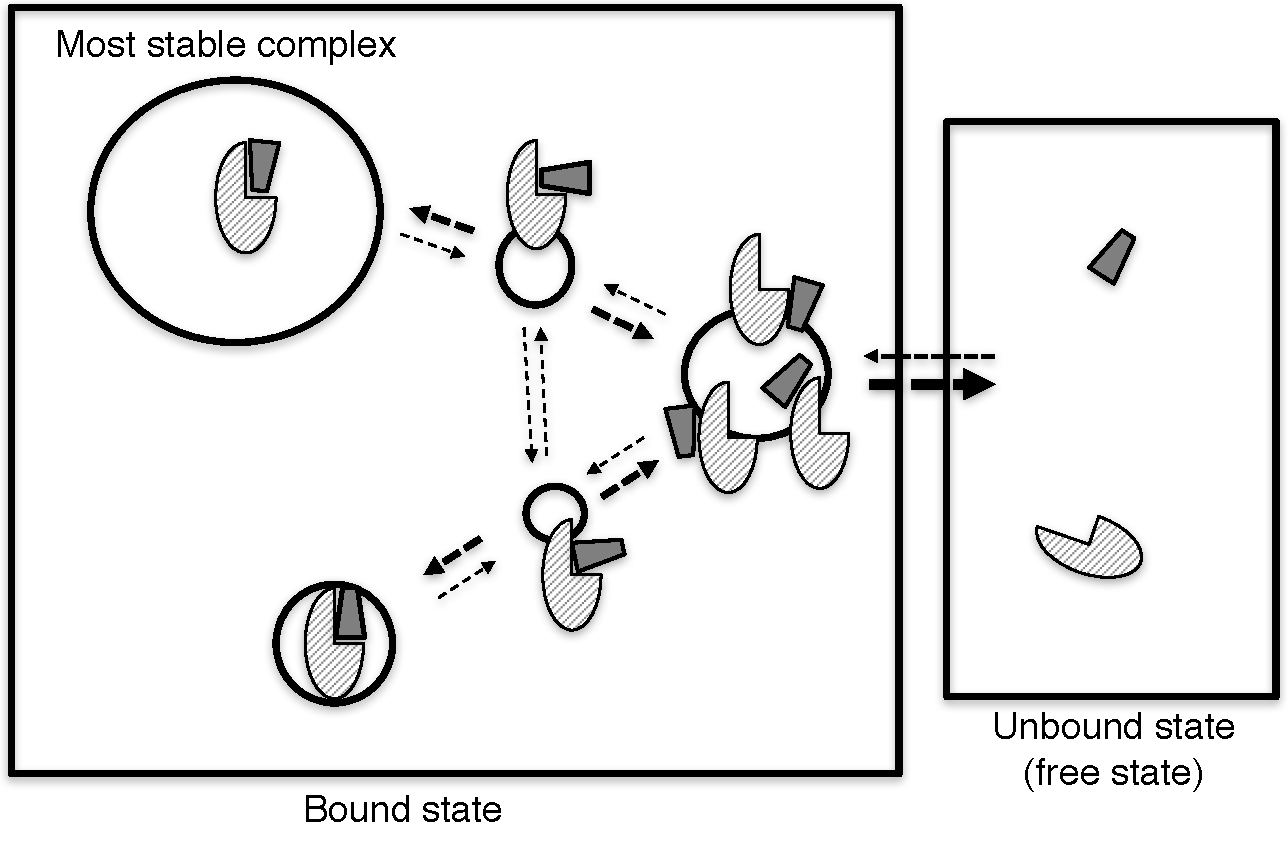
\includegraphics[width=10cm]{../enhance_rev/figures/u_b_states_pic.pdf}
  \caption{\label{fig:u_b_states_pic}}
\end{figure}

A quantitatively evaluated diagram is called a free-energy landscape and provides key information to discuss the complex formation in detail. Because conventional sampling methods have difficulty in obtaining an ensemble of snapshots enough to generate the free-energy landscape, several powerful computation methods have been developed. One way to approach the free-energy landscape is to use a powerful computer such as ANTON [3,4] or MDGRAPE [5] to perform a long time simulation. The second way is to integrate many simulation trajectories, where the trajectories generate a wide conformational distribution [6] or rate constant among conformational clusters [7,8], although each trajectory may cover only a small fraction of the whole conformational space. The third way is to use a generalized ensemble method [9,10]. In this review, we focus on various generalized ensemble methods that have been applied or are applicable to biomolecular binding with an atomistic resolution in an explicit solvent to obtain the free-energy landscape. Table 1 lists the generalized ensemble methods that are introduced in this review. We note that these methods are also applicable to large molecular conformational changes such as protein folding or intra-molecular conformational transitions by changing the computation object. In fact, many of the methods have been applied to folding in the referred papers.

In computational biophysics, development of an effective conformational sampling method has been one of the central subjects. When force field parameters are assigned to constituent atoms of the system (protein(s), ligand(s), and solvents), the potential energy is computable to the protein system. In this paper, potential energy is called “energy” simply. Different conformations of the system have different energy. Therefore, an energy surface (Figure \ref{fig:ene_landscape.pdf}a) can be constructed for the system in theory. Problems are: the energy surface of the protein system has a large number of energy basins surrounded by energy barriers, and some of conformational transitions among the basins are very slow processes. These difficulties arise as a result of the following factors: (i) The original conformational space is 3n-dimensional for a system consisting of n atoms, and n is usually large. (ii) Various types of interactions act among the constituent atoms. (iii) Usually there is no structural symmetry in the system. (iv) Motions of an atom are influenced strongly by the surrounding atoms because the atoms are densely packed. 
\begin{figure}
  \centering
  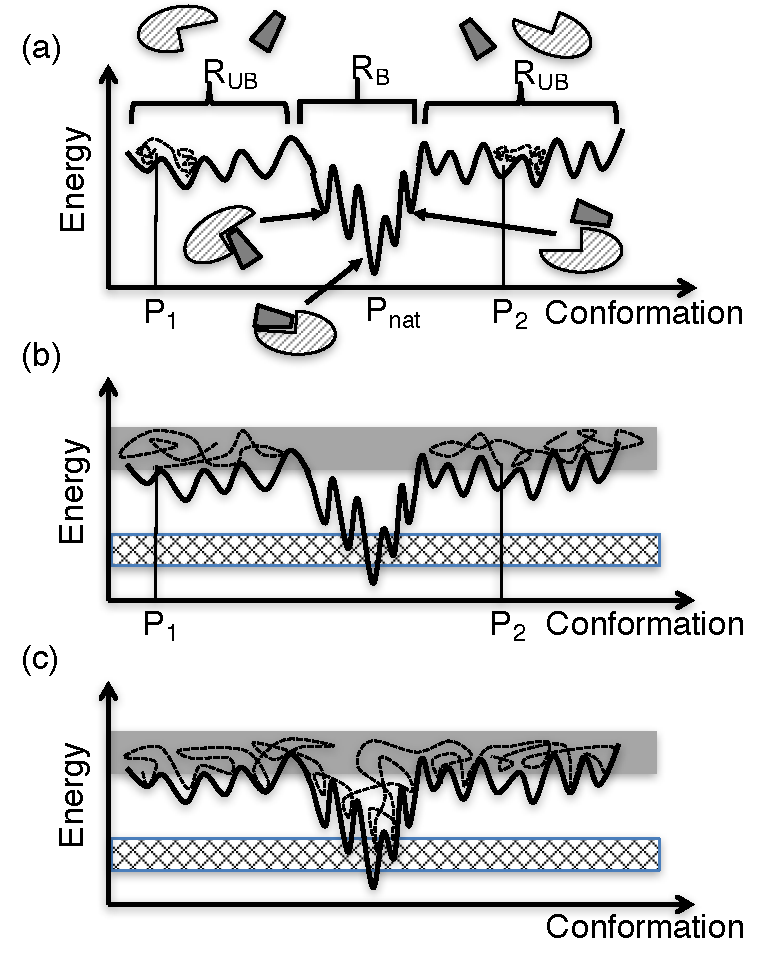
\includegraphics[width=10cm]{../enhance_rev/figures/ene_landscape.pdf}
  \caption{\label{fig:ene_landscape.pdf} Schematic representation of energy surface and simulation trajectories.
$X$- and $y$-axes represent conformation and energy for a two-molecular system,
respectively. Black curved line represents the energy surface, where energy minima and energy barriers distribute. Although the conformation of the system is defined originally in a high-dimensional space, the space shown in this figure is one-dimensional (i.e., $x$-axis). Molecular structures are also shown schematically. $\rm R_{\rm UB}$ is a region where unbound or slightly contacting molecules are distributed, and $\rm R_{\rm B}$ a region where various complex forms distribute. Although $\rm R_{\rm UB}$  is divided into two in this figure, they may be connected in the original high-dimensional space. (a) Broken lines represent simulation trajectories at room temperature starting from conformations at $\rm P_1$ and $\rm P_2$, which are far from the native complex structure ($\rm P_{\rm nat}$). The conformation moves slowly in the space because energy barriers interfere the motion. (b) Simulation trajectories (broken lines) at high temperature. The trajectories fluctuate in a high-energy range (shaded energy range), which involves $\rm R_{\rm UB}$, and the room-temperature range (checked range) is not sampled. Volume of $\rm R_{\rm B}$ is considerably narrower than that of $\rm R_{\rm UB}$ in the original high-dimensional space. (c) Trajectory from multicanonical simulation, which sample evenly the high and low energy ranges.}
\end{figure}

When one performs a molecular simulation at room temperature (denoted as $T_{\rm room}$ ), the conformation of the protein is usually trapped in energy basins near the initial conformation of the simulation (Figure \ref{fig:ene_landscape.pdf}a). Note that majority of proteins exert their biological functions at the room temperature, and then many biological experiments have been performed at this temperature. Then, to sample a wide conformational area with overcoming energy barriers and reach the native complex structure (i.e., experimentally determined complex structure at $T_{\rm room}$), a long simulation is required when the simulation starts from a dissociated conformation. A simple method to sample various conformations without being trapped is a high-temperature simulation (Figure \ref{fig:ene_landscape.pdf}b). This method, however, generates conformations accessible only at the high temperature. Inversely, when the high-temperature simulation starts from the native complex structure, this complex dissociates eventually, and the transition probability that the dissociated molecules rebind again to the native complex is negligibly small. A requirement imposed on the sampling method is that the resulted ensemble should consist of conformations probable at $T_{\rm room}$ in equilibrium (conformations in the checked energy range in Figure \ref{fig:ene_landscape.pdf}b) even when the simulation starts from a dissociated conformation. We denote this ensemble as $Q(T_{\rm room})$. The free energy landscape is derived from $Q(T_{\rm room})$. \textcolor{red}{@@@No (c)???}

The high-dimensional space to express the protein conformation is beyond our comprehension. Then, contraction of the high-dimensional space into a low-dimensional space is essential. Some parameters, such as relative molecular orientation of one molecule to the other, separation distance between two molecules, or root mean square deviation from a reference complex structure, are useful to construct the low-dimensional space for viewing the conformational distribution. Suppose that two parameters, denoted as  $s_1$ and$s_2$ , are selected for the coordinate axes of the contracted space (here it is a two-dimensional (2D) space). Then a set of parameters $[s_1, s_2]$ is calculated for all of the conformations stored in $Q(T_{\rm room})$, and a probability distribution function $P_{\rm cano}(s_1, s_2, T_{\rm room})$ is computed. A “potential of mean force (PMF)”, $F(s_1, s_2, T_{\rm room})$ , is formally defined as:
\begin{equation}
F(s_1, s_2, T_{\rm room})=-RT \ln [P_{\rm cano}(s_1, s_2, T_{\rm room})],
\label{eq:pmf}
\end{equation}
where $R$ is the gas constant. Equation \ref{eq:pmf} shows that a low PMF is assigned to a high-probability position. Note that high-probability regions in the conformational space are more stable thermodynamically than low-probability regions. In other words, the low-PMF regions are thermodynamically stable. Therefore, PMF is regarded as a free-energy landscape. The low-PMF regions are called “free-energy basins”, and the parameters $s_1$ and $s_2$ are called “reaction coordinates”. Figure \ref{fig:pmf_pic.pdf} illustrates the relation between $P_{\rm cano}$ and $F$ in one-dimensional case. In a general case, $P_{\rm cano}$ is converted as:
\begin{equation}
F(s_1,s_2,s_3,..,s_n, T_{\rm room})=-RT_{\rm room} \ln [P_{\rm cano}(s_1,s_2,s_3,..,s_n, T_{\rm room})],
\label{eq:pmf_gene}
\end{equation}
where both $P_{\rm cano}$ and $F$  are expressed by $n$ parameters.
\begin{figure}
  \centering
  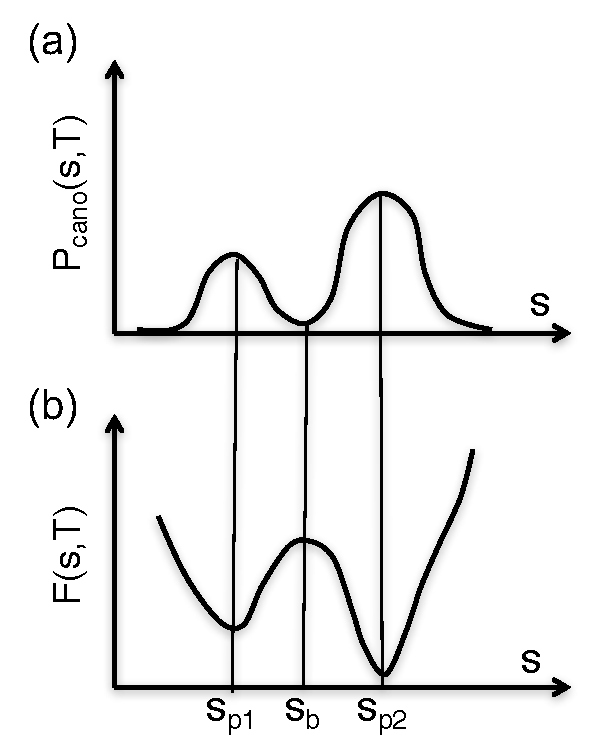
\includegraphics[width=10cm]{../enhance_rev/figures/pmf_pic.pdf}
  \caption{\label{fig:pmf_pic.pdf} Conversion of distribution function to PMF in one-dimensional case. One-dimensional parameter is denoted as $s$. (a) Distribution $P(s,T)$, and (b) PMF: $F(s,T)=-RT \ln[P(s,T)]$. High probability is assigned to $s_{\rm p1}$ and $s_{\rm p2}$, where $F(s,T)$ is low. Contrarily, the low-probability is assigned to $s_{\rm b}$, where $F(s,T)$ is high.}
\end{figure}

\section{Umbrella Sampling}
As an enhanced sampling method, we first introduce umbrella sampling [11,12]. In this method, an appropriate reaction coordinate $p$ is set in advance so that the variation of $p$ reflects well the change of complex form. Figure \ref{fig:us_picture.pdf}a shows schematically the $p$-axis, which connects the unbound ($p_u$) and the native-complex structures ($p_n$). The umbrella sampling method introduces bias functions called “umbrella potential functions” along the $p$-axis. A bias potential set at a bias center (one of the filled or open circles in Figure \ref{fig:us_picture.pdf}a) affects the conformation to be confined within a narrow region around the bias center during a simulation. Then, performing individual simulations at different bias centers at temperature $T_{\rm room}$, one can obtain a number of biased distribution functions (Figure \ref{fig:us_picture.pdf}b). The purpose of the umbrella sampling is to obtain an entire distribution function $P_{\rm cano}(p, T_{\rm room})$ without the effects of the bias potentials in the full range $[p_u,p_n]$ of the $p$-axis. Then a reweighting technique is applied on each of the biased distributions, and non-biased fragments of the entire distribution (Figure \ref{fig:us_picture.pdf}c) are obtained. Finally, smooth connection of the fragments produces $P_{\rm cano}(p, T_{\rm room})$ (Figure \ref{fig:us_picture.pdf}d). This connection technique is called a "weighted histogram analysis" [13]. After the simulations, sampled snapshots are also reweighted and integrated into the conformational ensemble $Q(T_{\rm room})$. 
\begin{figure}
  \centering
  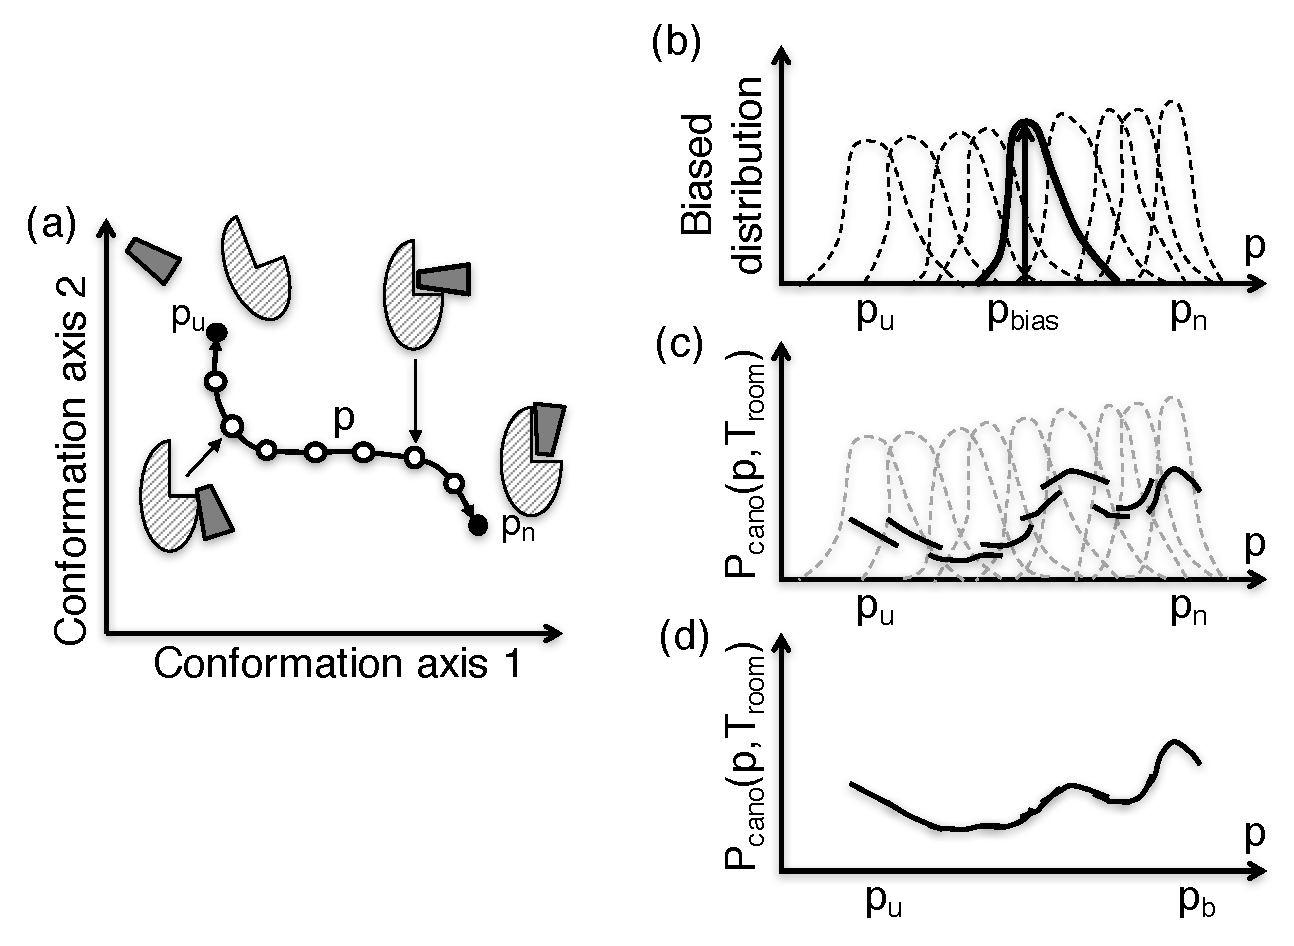
\includegraphics[width=10cm]{../enhance_rev/figures/us_picture.pdf}
  \caption{\label{fig:us_picture.pdf} Scheme for explaining umbrella sampling. (a) High-dimensional space is expressed here two-dimensionally ("conformational axis 1" and "conformational axis 2"), and reaction coordinate p is defined, for which the edges with filled circles labeled pu and pn correspond to unbound and native complex conformations, respectively. Open circles are intermediate conformations along the $p$-axis. (b) Biased distribution functions (broken and solid lines) obtained by individual simulations at different bias centers at temperature Troom . The solid line highlights a distribution around bias center pbias . (c) Solid lines are fragments of the full distribution function $P_{\rm cano}(p,T_{\rm room})$. Each fragment is computed only in well-sampled region of a biased distribution function in panel b.(d) $P_{\rm cano}(p,T_{\rm room})$ is obtained by smoothly connecting the fragments.}
\end{figure}

\section{Adaptive Umbrella Sampling}
“Adaptive umbrella sampling (AUS)” [14,15] also introduces a bias function. However, this bias function is not for restricting the conformation in a narrow range of the reaction–coordinate $p$. Contrarily, the bias assists the conformation to fluctuate in the range $[p_u, p_n]$ smoothly (Figure \ref{fig:dist_for_aus.pdf}a). In short, AUS is a method to enhance the conformational fluctuations along the reaction-coordinate. The bias potential $E_{\rm aus}$ is given as:
\begin{equation}
E_{\rm AUS} = E + RT_{\rm room} \ln [P_{\rm cano}(E,T_{\rm room})].
\label{eq:e_aus}
\end{equation}
Note that the second term of the right side of this equation is PMF (see Eqs. 1 and 2). An MD simulation at $T_{\rm room}$, where $E_{\rm AUS}$ is used for evaluation of inter-atomic forces ($force=-\nabla E_{\rm AUS}$), produces a flat distribution function  along the -axis (Figure \ref{fig:dist_for_aus.pdf}b) when the function  is accurate enough and the simulation is long enough: $P_{\rm AUS}(p,T_{\rm room}) \approx const$.
\begin{figure}
  \centering
  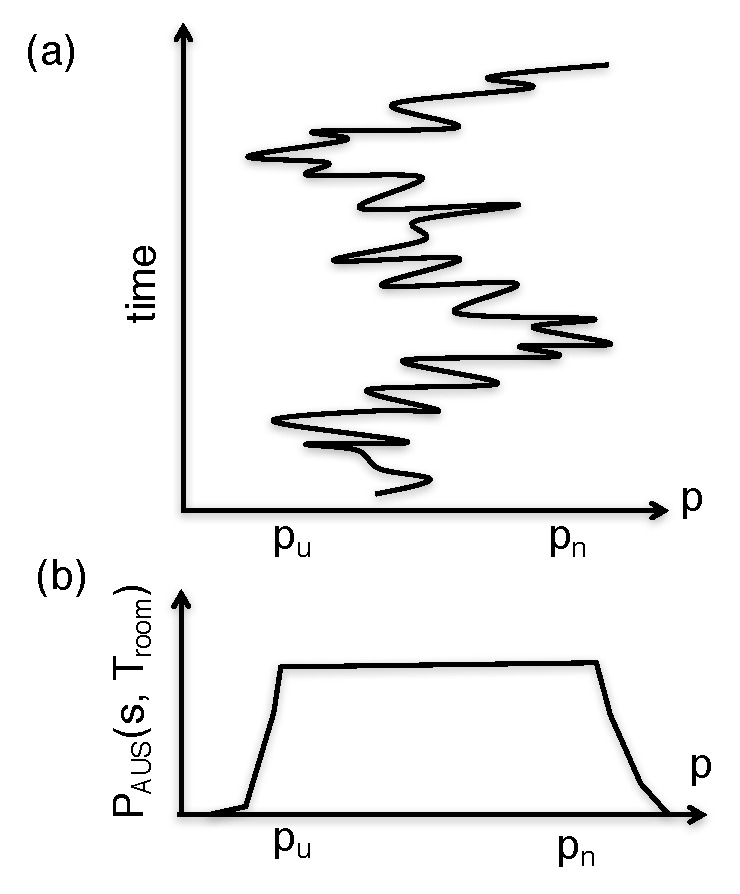
\includegraphics[width=10cm]{../enhance_rev/figures/dist_for_aus.pdf}
  \caption{\label{fig:dist_for_aus.pdf} Scheme for adaptive umbrella sampling (AUS). (a) The conformation fluctuates in range $[p_u, p_n]$ of reaction-coordinate axis $p$ with time. (b) Conformational distribution $P_{\rm AUS} (p ,T_{\rm room})$ resulted from AUS.}
\end{figure}

Note that the distribution function $P_{\rm cano}(E,T_{\rm room})$ is unknown in advance, and then, this function is refined iteratively through simulations [10]: After a simulation has been finished, $P_{\rm cano}(E,T_{\rm room})$ is updated from the simulation trajectory, and the next simulation is started using the updated function, and so on. Through the iterations, $P_{\rm AUS}(p,T_{\rm room})$ is flattened more and more, and when $P_{\rm AUS}(p,T_{\rm room})$ becomes flat enough, we judge that  is accurate enough. Finally, we perform a long simulation using the refined $P_{\rm cano}(E,T_{\rm room})$ and store snapshots. Then $Q(T_{\rm room})$ is generated where a thermal weight at $T_{\rm room}$ is assigned to each of the stored snapshots (reweighting).

\section{Metadynamics(Higo version)}
A method called “metadynamics” refines $P_{\rm cano}(E,T_{\rm room})$ within a simulation [16,17]. Thus, metadynamics is an iteration-free method and, thus, suitable for automation of simulation procedure [10]. Wang-Landau sampling [18], which enhances the conformational fluctuations along the energy axis as explained later, also refine a bias potential within a simulation.
\section{Metadynamics (Shinji version)}

\section{Multicanonical Sampling}
Multicanonical sampling was proposed originally to study statistical properties of a physical model, Potts model [19]. In this work, the Metropolis Monte-Carlo algorithm was carried out to explore the conformational space. Then, this method was applied to biological systems [20-23], and extended to an MD scheme where Newtonian equations were solved in the Cartesian coordinate space [24]. We denote this MD-based multicanonical method “McMD”. The adoption of the Cartesian coordinates makes the sampling applicable readily to a multi-polypeptide system in explicit solvent [25]. 

As with the adaptive umbrella sampling, multicanonical sampling introduces an energy bias function (multicanonical potential energy) as:
\begin{equation}
\label{eq:e_mc}
E_{\rm MC} = E + RT_{\rm room} \ln [P_{\rm cano}(E,T_{\rm room})],
\end{equation}
where $P_{\rm cano}(E,T_{\rm room})$ is the canonical energy distribution function at . An MD simulation using atomic forces of $force=-\nabla E_{\rm MC}$ at $T_{\rm room})$ produces a flat distribution function ($P_{\rm MC} \approx const$) along the energy axis when the function  is accurate enough and the simulation is long enough. Therefore, the multicanonical sampling enhances the fluctuations along the energy axis: When the system is in a high-energy range (the shaded range in Figure \ref{fig:ene_landscape.pdf}c), the conformation can overcome energy barriers, and when the system is in a low-energy range (the checked range in Figure \ref{fig:ene_landscape.pdf}c), which corresponds to the room-temperature range, the sampled conformations are accumulated into the ensemble $Q(T_{\rm room})$.

Recently, trajectory parallelization has been combined with McMD [6,26], and applied to a system consisting of a fragment taken from an intrinsically disorder protein and its partner protein in explicit solvent [27]. Furthermore, a virtual system, which has arbitral physical properties defined by a researcher, has been introduced to enhance sampling and coupled with the biomolecular system [28]. This procedure was named “virtual-system coupled multicanonical molecular dynamics (V-McMD)”. The V-McMD method was combined with the trajectory parallelization and applied to the p53 inter-domain linker, which is an intrinsically disordered region of p53 to regulate the p53–DNA interactions [29].

As well as the adaptive umbrella sampling, the distribution function $P_{\rm cano}(E,T_{\rm room})$ is unknown in advance. Then this function is determined iteratively: When the i-th simulation run has been finished, $P_{\rm cano}(E,T_{\rm room})$ is updated using a recurrent equation (see Ref. 10), $E_{\rm MC}$ is refined using Eq. \ref{eq:e_mc}, and the (i+1)-th run is performed. We call this procedure an “every-run” update method. As mentioned above, the Wang–Landau sampling method [18] updates $P_{\rm cano}(E,T_{\rm room})$ at every step of simulation. We call this updating method an “every-step” update method. A force-biased multicanonical MD [30] is a method in between the every-run and every-step update methods: A long simulation can be regarded as a succession of simulation intervals (blocks). After a block has been finished, $P_{\rm cano}(E,T_{\rm room})$ is updated using the data in this block, and the simulation for the next block is started using the updated $P_{\rm cano}(E,T_{\rm room})$. We call this method an “every-interval” update method. This method is also suitable for automating the simulation procedure.

\section{Simulated Annealing}
Not being a generalised ensemble method, simulated annealing methods, which has been applied to Monte Carlo and molecular dynamics simulations, can also search for energy minima in a potential energy surface of a physical system [ref]. 

The essential idea is the consideration of temperature of the system:
Increasing temperature of a physical system, the method makes a variety of configuration  accessible, and then it cools the system, thereby being able to search for an energy minimum. If we want to explore many energy minima, then SA simulations must be started with different initial configurations.

In general, it is said that the decrease speed of temperature should be slow in order to avoid becoming trapped in high potential energy regions and to explore thoroughly a potential surface {\color{red} [WHY THEY HAPPEN IF DO THAT?]}. However, {\color {red} FIXME there is no way to avoid the problems exactly.} Even in a rude cooling schedule, we may obtain a good result.

\section{Simulated Tempering}
Simulated tempering [31,32] is a method where temperature of the system changes as $T_1 \rightarrow T_2 \rightarrow T_3 \cdots$ during a simulation with satisfying the detailed balance condition at the temperature switching, and similar methods with the simulated tempering have been proposed [33-35]. In this method, temperature fluctuates covering a range from room to high temperatures. When the temperature is elevated, the system overcomes energy barriers. 

\section{Temperature Replica Exchange Method (Parallel Tempering)
{\color{red} (add figures to explain REMD)}
}
A method called “temperature replica exchange method (tREM)” [36,37] or “parallel tempering” [38] introduces multiple systems (replicas), whose chemical compositions are exactly the same one another, although the temperatures are different. These replicas evolve according to the Newtonian equations of motion (or Monte Carlo method) for a while, and occasionally exchange their temperatures imposing the detailed balance condition at the temperature exchange. Therefore, each replica experiences various temperatures during the time–evolution. Importantly, replicas overcome energy barriers when their temperatures are high. One of the temperatures is, at least, set to $T_{\rm room}$, and then, snapshots sampled at $T_{\rm room}$ are assembled in $Q(T_{\rm room})$. Lyman et al. expanded the replica exchange method where replicas are expressed by different resolution models, such as all-atom and coarse grained models, and the resolutions are exchanged among the replicas in a simulation [39]. In fact, the quantity to be exchanged is arbitral [40], and some exchange methods have been proposed: exchange of van der Waals radius [41], coulomb interactions [42], and Hamiltonian [43].

\section{$\lambda$-Dynamics}
A method called “$\lambda$-dynamics” [44,45] also enhances the conformational fluctuations along an arbitrarily structural parameter (the reaction–coordinate called $\lambda$) as with the adaptive umbrella sampling. In the $\lambda$-dynamics, however, the reaction–coordinate is treated as a dynamical quantity: I.e., $\lambda$ and its momentum  are involved as dynamical variables in the equations of motion. Ikebe et al. recently have proposed an extended form of $\lambda$-dynamics, adaptive lambda square dynamics (ALSD), where different weights are assigned to each energy term and the weights fluctuate as dynamical variables [46]. ALSD is effective to sample a biomolecular system where very strong and weak interactions are mixed [47].

\section{Suwa-Todo Algorithm}
In most of conformational sampling methods based on the Monte-Carlo scheme, the conformational changes are controlled by the detailed balance condition. Recently, an algorithm, called the Suwa-Todo algorithm [48], has been proposed based on a balance condition (non-detailed balance condition). Then probability fluxes may occur in time–evolution of the probability distribution function of the system. Importantly, an equilibrated distribution is obtained finally in spite that the detailed balance condition is broken. Based on the Suwa-Todo algorithm, biomolecular sampling methods have been proposed [49,50], where although the method has a similar fashion with the replica exchange method, the exchange (or permutation) rule among the replicas obeys the Suwa-Todo condition. These methods may generate a new trend in conformational sampling.

\section{Double Density Dynamics}
Double density dynamics (DDD) is a sampling method where an arbitrary parameter and its momentum are treated as dynamic variables in the equations of motion [51]. As a result, the parameter fluctuates in a given range. One may think that DDD has a similar fashion with the $\lambda$-dynamics or ALSD mentioned above. In DDD, however, the statistics to that microscopic states obey can be designed arbitrarily. Thus, one can optimize the sampling efficiency by modulating the statistics in theory.

\chapter{Applications of a GE method to NRSF-Sin3 and Endthelin-1 derivative}
We mentioned in the introduction-section that the generalised ensemble method elucidates not only the most thermodynamically stable state (the largest conformational cluster) but also semi-stable states, which may appear temporally in the molecular binding process. We shall introduce our recent computational study on an intrinsically disordered protein (IDP) interacting to its partner protein. IDP is a challenging system to examine the efficiency of the generalized ensemble methods because IDPs have larger conformational fluctuations than ordered proteins (regular proteins). Therefore, the free-energy landscape of IDP consists of both the most stable and semi-stable states. 

\begin{figure}
  \centering
  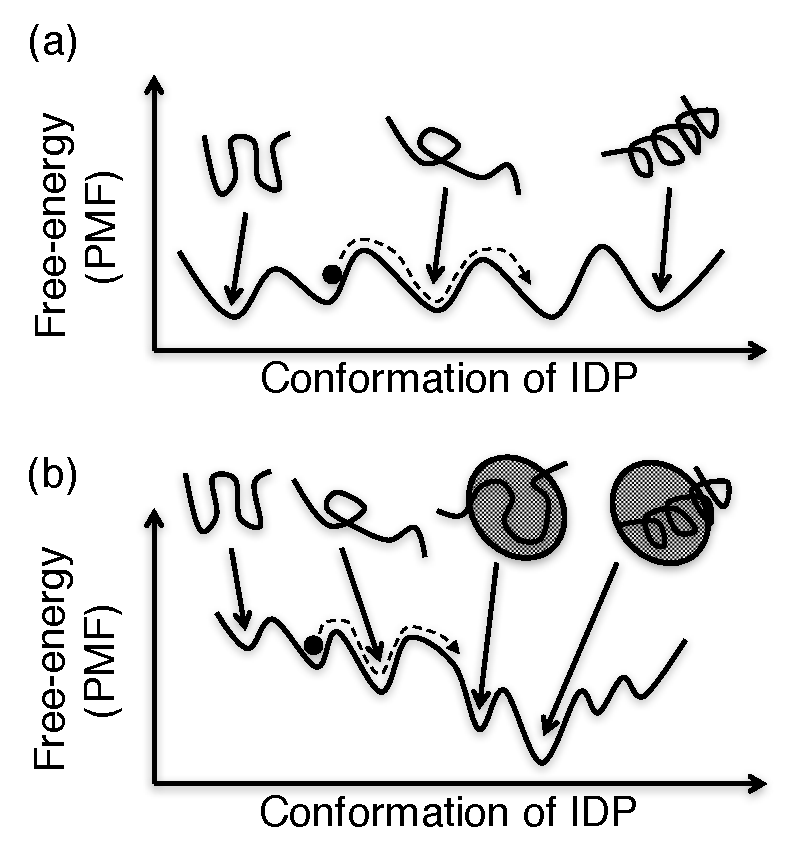
\includegraphics[width=10cm]{../enhance_rev/figures/fel_idps.pdf}
  \caption{\label{fig:fel_idps.pdf} Schematic free-energy landscape of IDP in (a) unbound and (b) bound states shown one-dimensionally. $X$-axis represents conformation of IDP, although the system in panel (b) consists of two molecules (IDP and its partner). Black filled circle represents the IDP conformation moving along simulation trajectory (broken line).}
\end{figure}
An ordered protein has its own tertiary structures (native structure) determined by its aminoacid sequence, and the tertiary structure does not vary largely before and after the complex formation. Contrarily, a unique tertiary structure is not assigned to IDP when the IDP is in the unbound state (isolated state), and the unique structure is formed when it binds to its partner molecules [52-54]. This mechanism is known as “coupled folding and binding” [54]. Therefore, the free-energy landscape of IDP in the unbound state has no dominant cluster prevailing against the other clusters (Figure \ref{fig:fel_idps.pdf}a). In the bound state, contrarily, the landscape has the dominant cluster (the most stable complex) (Figure \ref{fig:fel_idps.pdf}b).

We have computed the free-energy landscape of two systems: NRSF–mSin3 [27] and pKID-KIX [55] systems, where NRSF and pKID are IDPs, and mSin2 and KIX are their partner proteins. In this review, we focus on the NRSF–mSin3 system. NRSF (the N-terminal repressor domain of neural restrictive silencer factor) is an IDP known as an essential transcriptional repressor for neuron-specific genes in non-neuronal cells and neuronal progenitors, and mSin3 is its partner protein. The complex structure was solved by an NMR experiment [56], where a 15-residue segment of NRSF fragment folded into helix when bound to the cleft on the surface of the paired amphipathic helix (PAH) domain of mSin3. The regions of NRSF other than the 15-residue segment are disordered even in the complex structure.

In the McMD simulation, the 15-residue fragment and the PAH domain of mSin3 were treated. We denote the PAH domain of mSin3 simply as mSin3. In the initial conformation of the simulation, these two molecules were distant to each other in an explicit solvent. Furthermore, the conformation of the NRSF segment was disordered in advance (Figure 1c in Ref. 27). After the refinement of multicanonical energy $E_{\rm MC}$ (Eq. \ref{eq:e_mc}) via iterative McMD simulations, production runs were performed yielding the ensemble $Q(300 K)$. McMD of the single NRSF fragment (i.e., unbound state) was also performed with a similar simulation procedure. The initial conformation of the NRSF fragment was randomized in advance and put in an explicit solvent (Figure 1b in Ref. 27).

\begin{figure}
  \centering
  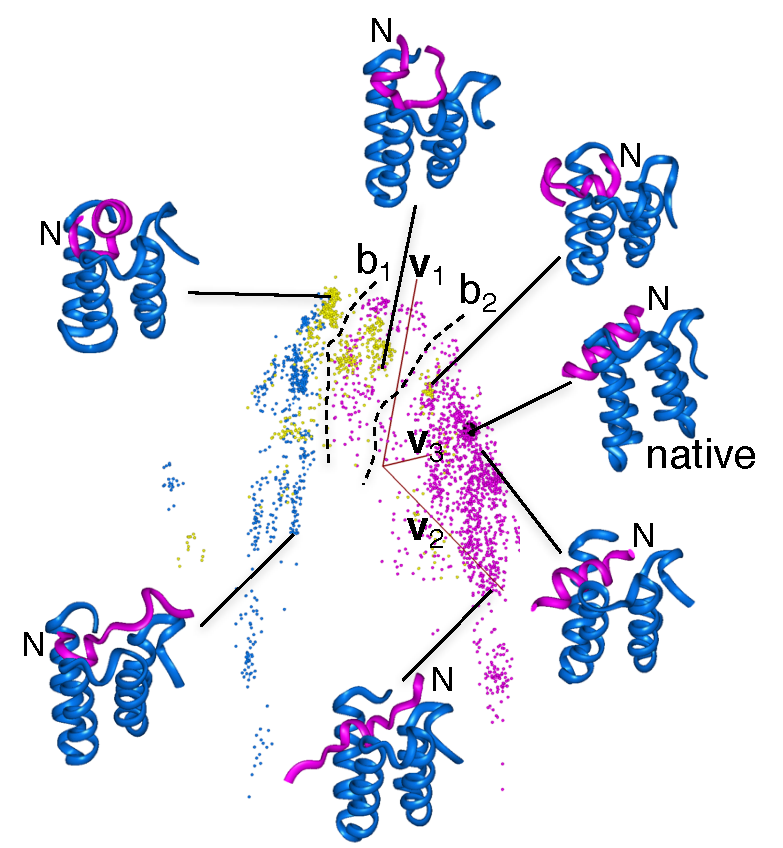
\includegraphics[width=10cm]{../enhance_rev/figures/msin_nrsf_fel.pdf}
  \caption{\label{fig:msin_nrsf_fel.pdf} (a) Conformational distribution of $Q$(300 K) for system consisting of the NRSF fragment and mSin3. The distribution is shown in an abstract thee-dimensional (3D) space, whose coordinate axes (orange-tan colored lines), labeled $\bm{\nu}_1$, $\bm{\nu}_2$ and $\bm{\nu}_3$, are calculated from a principal component analysis (PCA): Each colored dot is projection of a conformation of the NRSF fragment in the 3D space (see Ref. 27). The closer the two dots, the similar the two conformations. Some tertiary structures are also displayed, where magenta model is the NRSF fragment and blue model is mSin3. Yellow spheres indicate the N-terminus of the NRSF fragment. Black sphere represents the position of the NMR complex structure labeled by “native”. There are three large domains spaced by broken lines labeled b1 and b2, along which dots distribute sparsely. Dots are colored depending on mutual molecular orientations between the two molecules: The color is magenta when the NRSF fragment is approximately parallel to the cleft of mSin3, and the color is cyan when they are approximately anti-parallel. Otherwise, the color is yellow. See Ref. 27 for strict coloring method.
}
\end{figure}
Conformational clustering applied to $Q(300 K)$ has shown that the largest cluster (i.e., the most stable cluster) is the native-like complex cluster (Figure \ref{fig:msin_nrsf_fel.pdf} in Ref. 27). Thus, the McMD simulations provided reliable data in the sense that the NMR complex was predicted correctly. In a high-energy range, the NRSF fragment distributed widely in space without a dominant structure (Figure 4A in Ref. 27). Contrarily, at 300 K, the NRSF segment was trapped into the NRSF binding cleft of mSin3 (Figure 4B in Ref. 27). Figure \ref{fig:msin_nrsf_fel.pdf} demonstrates the conformational distribution for $Q(300 K)$ projected in an abstract conformational space. Note that a region with crowded dots (conformations) corresponds to a low free-energy (PMF) region (see Eq. \ref{eq:pmf_gene}). Figure \ref{fig:msin_nrsf_fel.pdf} shows that three domains of crowded dots exist and that the domains were spaced by broken lines labeled b1 and b2, along which the dots distribute sparsely. These sparse-dot regions correspond to free-energy barriers because the probability of conformation around the regions is low. The domains were discriminated well by the molecular orientation of the NRSF fragment in the NRSF binding cleft of mSin3 (see figure legend). Therefore the rearrangement of the molecular orientation of the fragment requires jumping the free-energy barriers. 

\begin{figure}
  \centering
  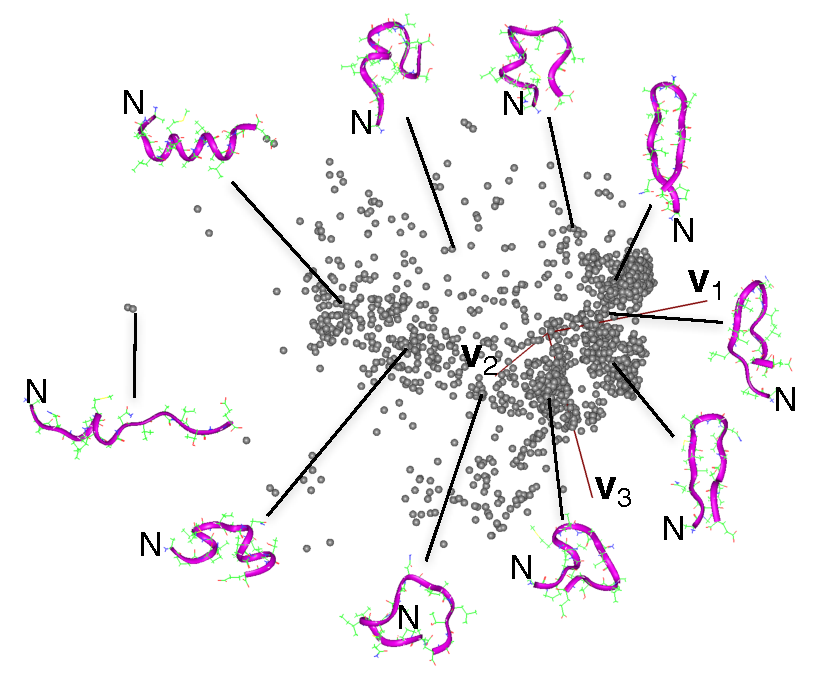
\includegraphics[width=10cm]{../enhance_rev/figures/msin3_fel.pdf}
  \caption{\label{fig:msin3_fel.pdf} Conformational distribution of $Q$(300 K) for single NRSF fragment. Axes $\bm{\nu}_1$, $\bm{\nu}_2$ and $\bm{\nu}_3$ are calculated as with Figure \ref{fig:msin_nrsf_fel.pdf}. Some conformations are also displayed. Yellow spheres indicate the N-terminus of the NRSF fragment.}
\end{figure}
Figure \ref{fig:msin3_fel.pdf} represents the conformational distribution of $Q(300 K)$ for the single NRSF fragment. A variety of conformations, such as helix, hairpin, bent, etc., are seen in the conformational space, which means that the conformation fluctuates among these structures in solution at 300 K: No dominant structure exists. Therefore the NRSF fragment is disordered in the unbound state. Interestingly, most of conformations in  of the single-NRSF system are found in that of the NRSF-mSin3 system, whereas the probabilities assigned to the conformations are different between the two systems (Figure 10 in Ref. 27). The main feature for the complex state was helix, although the single NRSF fragment adopts both the helix and hairpin (Figure 3 in Ref. 27).

From these results, we have proposed a binging mechanism for the coupled folding and binding of NRSF (Figure \ref{fig:msin3_nrsf_regime.pdf}): In the unbound regime, NRSF fluctuates among various conformations. NRSF binds with the cleft of mSin3 with using these conformations, and non-native complexes are formed. The NRSF conformation moves in the bound regime. Otherwise the complex dissociates. Depending on the first formed non-native complex, the complex may overcome one or two free-energy barriers, and finally the native complex is formed. The McMD simulation has shown that the complex formation with the all-atom model is considerably complicated, where the complex experiences various intermediates overcoming free-energy barriers.
\begin{figure}
  \centering
  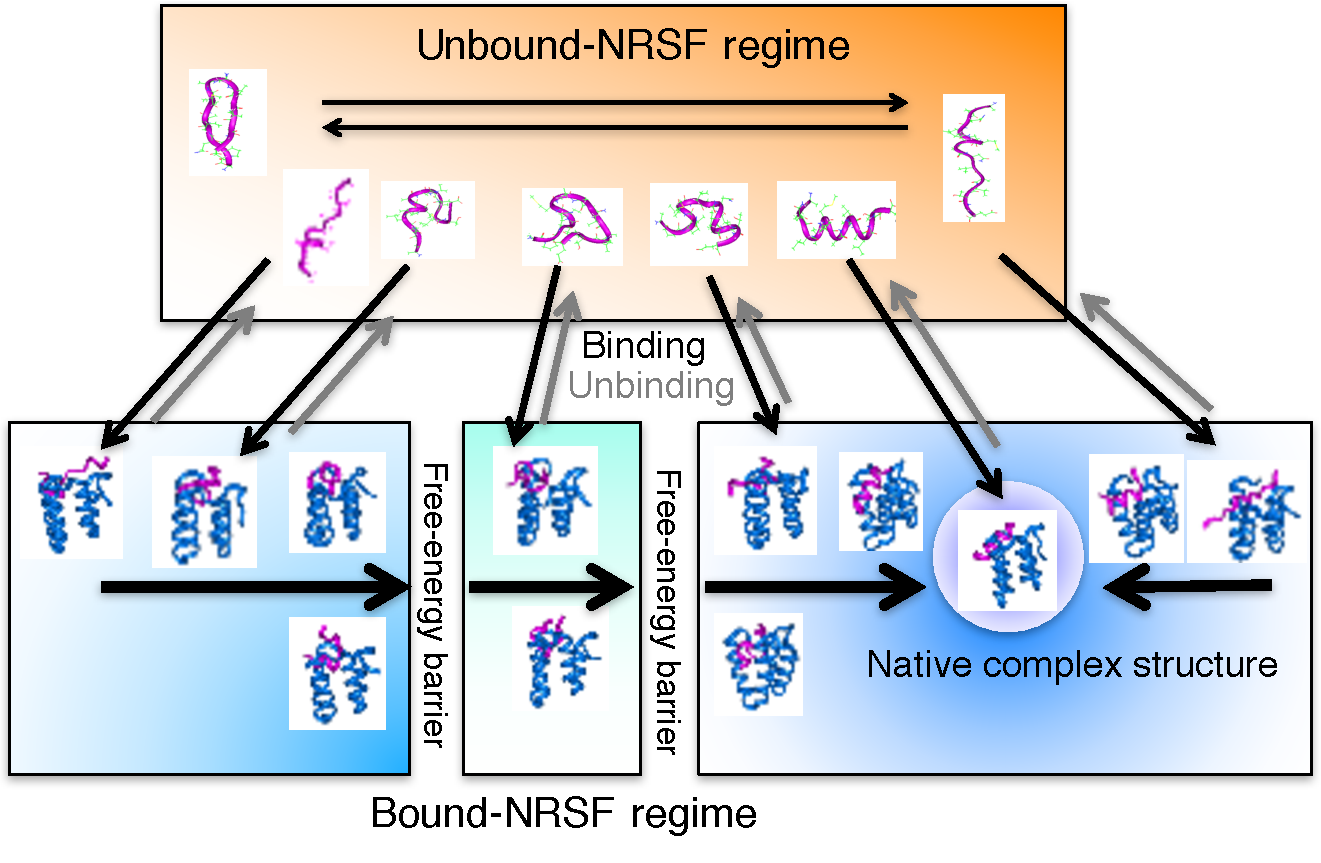
\includegraphics[width=10cm]{../enhance_rev/figures/msin3_nrsf_regime.pdf}
  \caption{\label{fig:msin3_nrsf_regime.pdf} Simplified free-energy landscape integrated from the all-atom detailed free-energy landscapes for the NRSF-mSim3 complex and single-chain NRSF. Arrows represent conformational changes. Yellow spheres in the molecular models indicate the N-terminus of the NRSF fragment.}
\end{figure}

\section{Virtual-system coupling}
Above we have introduced various enhanced conformational sampling methods. Now we introduce a "virtual system", which couples with the biomolecular system (restated as "real system") [57]. The entire system is a sum of the real system and the virtual system, which are specified by the coordinates $\bm{x}$ for the real system (i.e., coordinates of the constituent atoms of the molecular system) and a state parameter for the virtual system. In a simulation, both the real and virtual systems move. Advantageously, one can set the virtual system in an arbitrary manner. We trace the time–development of the entire system instead of pursuing the motions of the real system only. Recently, the virtual-system was integrated with McMD and AUS, which are abbreviated as "V-McMD" [28] and "V-AUS" [58], respectively. Although it may be difficult to understand intuitively the coupling between the real and virtual systems, the computational technique is simple as explained below. See Ref. 28 in detail.

\begin{figure}
  \centering
  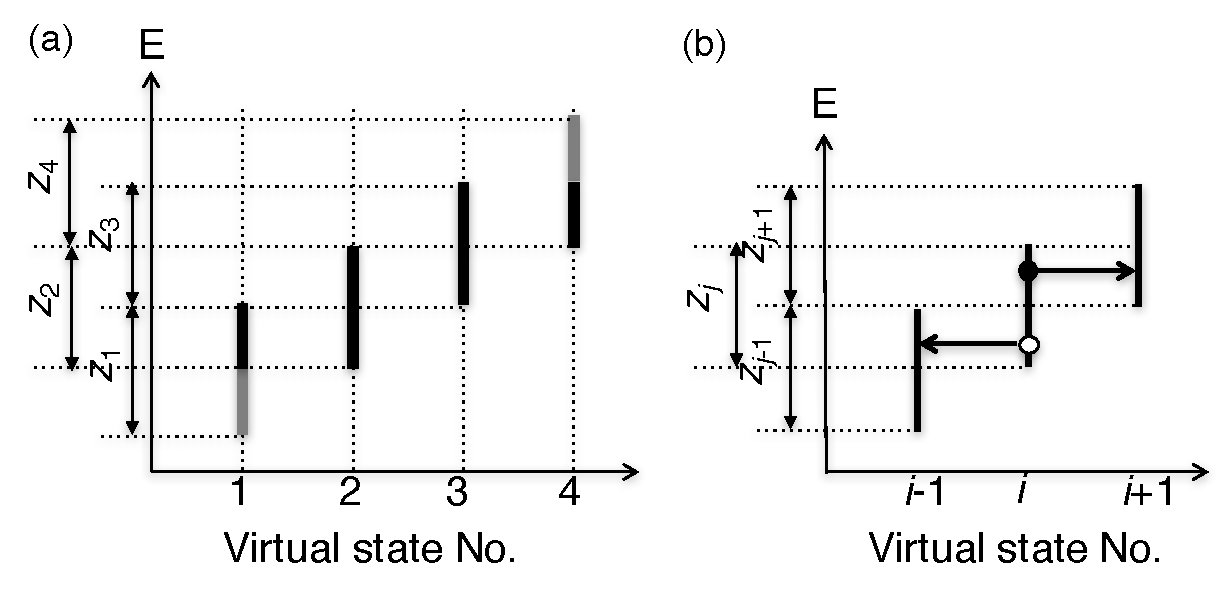
\includegraphics[width=10cm]{../enhance_rev/figures/vstate_transi.pdf}
  \caption{\label{fig:vstate_transi_fig} (a) Space constructed by the energy axis and virtual-state axis, where four virtual states exist as an example. Although the widths of the zones are shown equally in this figure, they are not necessarily the same in the actual sampling. (b) Transitions among adjacent virtual states. See text.}
\end{figure}
Imagine a virtual system, for which the state is specified by a discrete ordinal number  (“virtual-state index”). We assume that when the virtual-state index is $i$, the energy of the real system $E(\bm{x})$ is confined in an energy zone $z_i$ as: $z_i = [E^{\rm min} \leq E_i  \leq E^{\rm max}]$. Figure \ref{fig:vstate_transi_fig}a represents a space constructed by the energy axis and virtual-state axis. Zones $z_{i-1}$ and $z_i$ ($z_1$ and $z_2$ for instance) overlap to each other as well as $z_i$ and $z_{i+1}$ ($z_2$ and $z_3$ for instance) do, although two zones $z_{i-1}$ and $z_{i+1}$ do not overlap because the zones are set as: $[E^{\rm min}_{i+1} - E^{\rm max}_{i-1}] > \epsilon$, where $\epsilon$ is a positive but an infinitely small number. In time-development of the entire system, the conformation of the real system varies according to the equations of motion, and the virtual-state index jumps from $v_i$ to $v_{i+1}$ or $i-1$, by which the variable energy range for the real system is reset. If inter-virtual state transitions are exhibited in the simulation, the real system fluctuates within $z_i$, which means that only a narrow region of the conformational space is sampled (i.e., sampling efficiency is low). We define the inter-virtual state transitions as follows: Suppose that $E$ is at the filled-circle position in Figure \ref{fig:vstate_transi_fig}b. Then the virtual state $i$ may jump to the virtual state $i+1$ without changing $\bm{x}$ of the real system. On the other hand, if $E$ is at the open-circle position, the virtual state may transition to $i-1$. Then, we introduce a rule: during a time interval of $[t,t+\tau]$, the virtual state number is fixed to $i$, and $\bm{x}$ moves according to the ordinary equations of motion with confining $E$ in $z_i$. At time $t+\tau$ the transition is achieved to $z_{i-1}$ or $z_{i+1}$ with the transition probability  $\rho_t$ ($0 \leq \rho_t \leq 1$), at which $\bm{x}$ does not move. Due to the arbitrary property of the virtual system, one can set arbitrarily the transition probability $\rho_t$ and the interval $\tau$, which may increase the sampling efficiency [28,57]. Consequently, with traveling the virtual states, the real system fluctuates the wide conformational space overcoming energy barriers. The detailed balance for this time–development is theoretically well satisfied as described in APPENDICES. Introduction of the virtual system to AUS is explained in Ref. 58. 

Recently, Moritsugu et al. introduced “multiscale essential sampling (MSES)”, where a protein system was expressed by an all-atom model, and coupled with a coarse-grained (CG) model(s) to enhance conformational sampling [59,60]. MSES was applied to protein-protein binding of a barnase-barstar system [61]. The free-energy landscape for association/dissociation demonstrated existence of the non-native complex forms as well as the native-complex. Although the methodological fashion of MSES is considerably different from the virtual-system coupling method, the two methods have a similarity in the introduction of non-realistic systems to be coupled with the real system.

\section{A free energy landscape for dimer formation by V-McMD \label{et1_sec}}
Here, as an example of generalized ensemble method applied to a biomolecular complex formation, we show the free-energy landscape of homo-dimer formation of an endothelin-1 (ET1) derivative computed by V-McMD simulations. ET1 is a biomolecule of 21 aminoacids long known as a strong vasoconstrictor on smooth muscles of a vessel [62-64]. This molecule is a potent drug target because it is related to many human diseases [65-69]. The tertiary structure was solved by NMR spectroscopy [70-72] and X-ray crystallography [73]. In either study, the N-terminal region adopts a strand and the middle region forms an $\alpha$-helix. Because two disulfide bonds link the strand and the helix, the tertiary structure is compact and stable regardless of its short polypeptide length. 

\begin{figure}
  \centering
  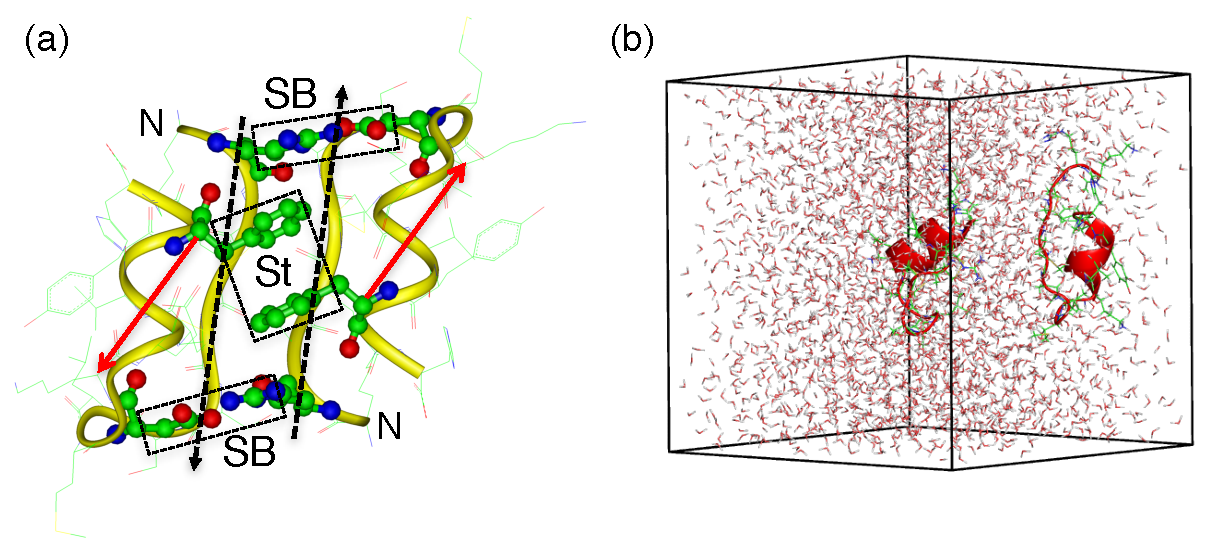
\includegraphics[width=10cm]{../enhance_rev/figures/et1_conf.pdf}
  \caption{\label{fig:et1_conf_fig} Homo-dimer complex of KR-CSH-ET1 determined by X-ray crystallography. Two “N” characters indicate the N-termini of the molecules. Inter-molecular $\beta$-sheet is formed between two strands indicated by black broken-line arrows. Inter-molecular hydrophobic stacking between phenylalanine side-chain rings is shown by the rectangle labeled “St”. Two inter-molecular salt bridges, formed between arginine and aspartic acid, are indicated by the rectangles labeled “SB”. Red arrows are used for identifying the molecular orientations of the two molecules, which point from the C$\alpha$ atom of Lys to the C$\alpha$ atom of the last Cys in the sequence of KR-CSH-ET1. (b) Initial conformation of V-McMD simulation.}
\end{figure}
ET1 aggregates at concentration of 1-4 mM. Then, to increase the solubility the N-terminal was extended by two charged aminoacid residues, Lys and Arg [74], which exist in its precursor protein. This extended ET1 is denoted as KR-ET1. Unexpectedly and interestingly, KR-ET1 has less activity than ET1 does in spite of increment of solubility. Then, an X-ray crystallography [75] showed that KR-ET1 forms a homo-dimer (PDBID; 1t7h) (Figure \ref{fig:et1_conf_fig}a), where the orientations of the two molecules are anti-parallel to each other although its molecular tertiary structure is similar with the single ET1 structure. In the study, five aminoacid residues at the C-terminal of KR-ET1 were removed because those residues are presumably disordered and exposed in solution. This truncated peptide of 18 aminoacids long (sequence: KRCSCSSLMDKECVYFCH) is denoted as KR-CSH-ET1. Figure \ref{fig:et1_conf_fig}a indicates that this complex is stabilized by three factors: inter-molecular $\beta$-sheet, inter-molecular hydrophobic stacking of phenylalanine side-chain rings, and two inter-molecular salt bridges. Therefore, the experimental study of Ref. 75 reported that this homo-dimer structure is considerably stable.

The dimer formation of KR-CSH-ET1 is an appropriate target for assessing V-McMD because the complex form is discriminated well by two quantities: the mutual molecular orientation $\bm{e}_{a1} \cdot \bm{e}_{a2}$ and the inter-molecular separation distance $r_{12}$, whose exact definition is given later. Previously we performed V-McMD simulations for KR-CSH-ET1 dimer formation [28], where the two molecules were confined in a spherical droplet of an explicit solvent, and the two-dimensional free-energy landscape was computed. The free-energy landscape at room temperature was predominantly composed of the crystallographic native complex structure. In the current review, we performed V-McMD of KR-CSH-ET1 dimer formation with periodic boundary condition, and computed the free-energy landscape. 

The simulation system was generated as follows: One KR-CSH-ET1 was immersed at the center of a periodic box (box size:  $45.000^3 \AA^3$) filled by an explicit solvent, and the other KR-CSH-ET1 was put at a position apart from the first KR-CSH-ET1 molecule. The system consisted of 8706 atoms (580 atoms for the KR-CSH-ET1 molecules, 9 Na+, 11 Cl- ions, and 2702 water molecules). The number of ions was determined to set the solution at a physiological salt concentration. Then a constant-pressure MD simulation (i.e., NPT simulation) was performed at room temperature and pressure of 1.0 atm, by which the initial conformation for V-McMD was prepared (resultant box size: $44.004^3 \AA^3$) (Figure \ref{fig:et1_conf_fig}b). The V-McMD simulation procedure was similar with that for the previous study [28] as follows: First refinement of $E_{\rm MC}$ was done via iterative V-McMD simulations, and then the production V-McMD simulation was performed to produce an entire conformational ensemble. The conformational ensemble $Q(T_{\rm room})$ was constructed by reweighting the snapshots in the entire ensemble. 

In V-McMD the energy moves in a wide range as mentioned previously. Then, KR-CSH-ET1 may unfold when the system is elevated to a high-energy region. The purpose of the current study is to show the free-energy landscape for the molecular binding, and refolding of KR-CSH-ET1 is outside the scope. Thus, we restrained weakly the tertiary structure of each KR-CSH-ET1 by intra-molecular restraint functions (see Ref. 28 for technical details). Thus, translational and rotational motions of the KR-CSH-ET1 molecules were free with maintaining their tertiary structures.

In this study, we set $T_{\rm room}$=300 K and obtained a canonical ensemble . Figure 12a demonstrates a free-energy landscape at 310 K presented two-dimensionally by $\bm{e}_{a1} \cdot \bm{e}_{a2}$ and $r_{12}$, whose exact definition is given in the figure legend. From this figure, the largest cluster (i.e., the lowest free-energy cluster) is native-like, where the two KR-CSH-ET1 molecules are arranged in anti-parallel, and the three factors, mentioned above, stabilized the complex structure. We call this cluster the native-like cluster. The landscape provided two other clusters. In the second largest cluster (the second lowest free-energy cluster), the orientations of the two KR-CSH-ET1 molecules are perpendicular to each other approximately: $\bm{e}_{a1} \cdot \bm{e}_{a2} \approx 0$. The third largest cluster (the third lowest free-energy cluster) was characterized by $\bm{e}_{a1} \cdot \bm{e}_{a2} \approx 1$, which means that the relative orientations of the two molecules are parallel. In the solvent-droplet boundary condition [28], the free-energy landscape had only the native-like cluster. It is likely that the solvent-droplet boundary condition would result in a stronger pressure than 1 atm in the droplet center due to the surface tension of the spherical droplet. This strong pressure could stabilize the well-packed conformation (i.e., native complex), and then probabilities assigned to the non-native complexes were diminished. The periodic boundary condition does not induce such an artificial excess pressure because there is no free surface in this treatment.

\begin{figure}
  \centering
  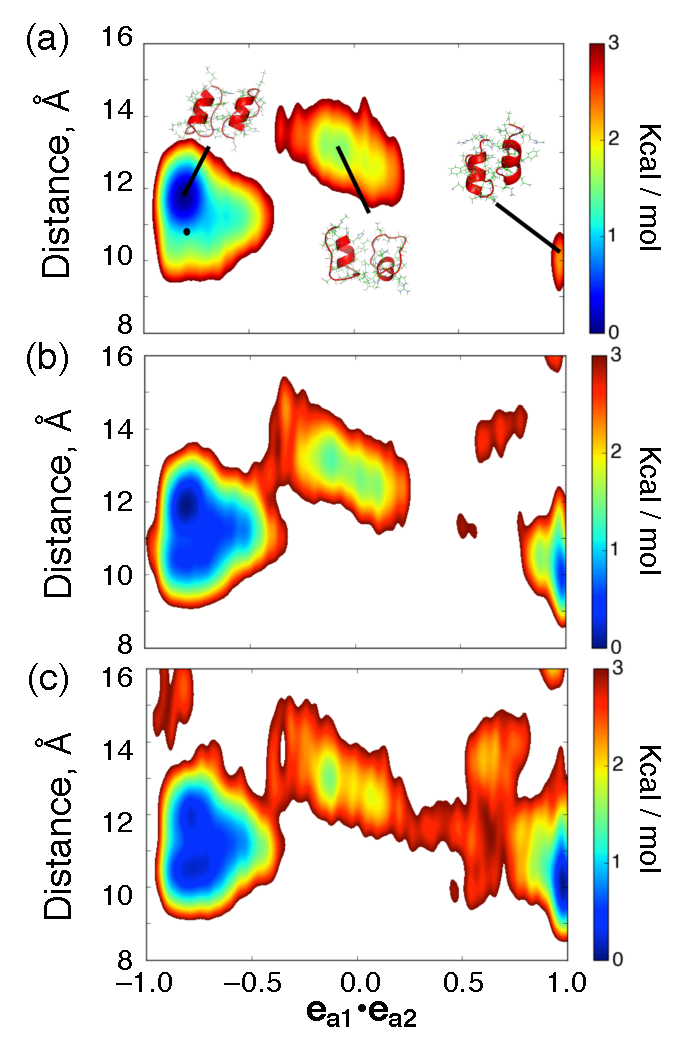
\includegraphics[width=10cm]{../enhance_rev/figures/dimer_form_fel.pdf}
  \caption{ \label{fig:dimer_form_fel_fig} 
Free-energy landscapes at (a) 310 K, (b) 350 K, and (c) 370 K. X-axis is mutual molecular orientation $\bm{e}_{a1} \cdot \bm{e}_{a2}$, where $\bm{e}_{a1}$ and $\bm{e}_{a2}$ are unit vectors parallel to the red-colored vectors in defined in Figure \ref{fig:et1_conf_fig}a: $-1 \leq \bm{e}_{a1} \cdot \bm{e}_{a2} \leq1$. Orientations of two KR-CSH-ET1 molecules are approximately parallel, anti-parallel, and perpendicular to each other for $\bm{e}_{a1} \cdot \bm{e}_{a2} \approx 1$, $\bm{e}_{a1} \cdot \bm{e}_{a2} \approx -1$, and $\bm{e}_{a1} \cdot \bm{e}_{a2} \approx 0$, respectively. Y-axis is inter-molecular separation distance $r_{12}=|\bm{r}_{G1}-\bm{r}_{G2}|$, where $\bm{r}_{G1}$ and $\bm{r}_{G2}$ are positions of the geometrical centres of the two molecules, and the geometrical centre is computed from the C$\alpha$-atomic positions of each molecule. The free-energy value (PMF; Eq. 1), whose height is shown by the coloured scale bars, is set so that the lowest PMF is zero. Tertiary structures from three clusters at 300 K are shown in panel (a), where the small black filled circle indicates the position of the native complex experimentally determined.}
\end{figure}

Figures \ref{fig:dimer_form_fel_fig}b and c demonstrate free-energy landscapes at 350 K and 370 K, respectively. The largest and second largest clusters are connected at 350 K, although the third largest cluster is still isolated. At 370 K, the third largest cluster is connected to the second largest cluster. We presume that once a non-native complex is formed in the cluster of $\bm{e}_{a1} \cdot \bm{e}_{a2} \approx 0$ , this complex can transition to the native-like cluster relatively readily. Contrarily, once a non-native complex is formed in the cluster of $\bm{e}_{a1} \cdot \bm{e}_{a2} \approx 1$, this complex should overcome a high-energy barrier to reach the native-like cluster via the cluster of $\bm{e}_{a1} \cdot \bm{e}_{a2} \approx 0$ . Otherwise, this complex dissociates, and the free KR-CSH-ET1 molecules may re-associate after that. Another interesting result from Figure \ref{fig:dimer_form_fel_fig} is that the second largest cluster at 300 K and 350 K is the third largest cluster at 370 K.

We exemplify in this section that the generalized ensemble method is a powerful tool to compute the free-energy landscape, by which we can discuss the thermodynamic stability of the clusters, the cluster networks, and the temperature dependence of the networks.

\section{Concluding remarks}
In this review, we introduced various generalized ensemble methods especially focusing on methods applicable to biomolecular association/dissociation with an atomistic resolution in explicit solvent to obtain the free-energy landscape. For making the methods useful for drug-discovery, the methods should not only explain basic mechanisms for association/dissociation, but also predict the complex forms and their stabilities. From this point of view, the sampling methods are useful if they generate a free-energy landscape for complex formation in explicit solvent at the atomistic resolution. In the introduction-section, we listed three approaches: fast computations, multiple simulation runs, and generalized ensemble methods. Note that these approaches can be combined. For instance, trajectory parallelization has been used for multicanonical and adaptive umbrella sampling. The free-energy landscape obtained from the generalized ensemble method does not involve information on rate constants. However, from the knowledge about the locations of many locally stable states, it is possible to look for the shortest path between a pair of conformational clusters, for example, by the string method [76], and the activation energy overcoming the energy barrier can be computed. In addition, combination of the generalized ensemble methods with the rate-constant estimation method using the Markov state model [7,8] among conformational clusters may be useful. 

In living matter, a number of biological molecules (proteins, metabolites, and DNAs) are crowding in solution (water and ions). Recent studies are revealing that crowding itself provides and/or enhances activities of the biomolecules [77, 78]. These large-scale studies, however, view the biomolecules neglecting their atomic details. Therefore, detailed intermolecular information from the generalized ensemble methods is useful to complete the molecular picture for living matter. 

Most of MD simulations currently used are based on the classical mechanics (Newtonian dynamics). On the other hands, many important processes taking place in living matter, such as catalytic reactions, are quantum chemical. Thus, development of quantum-mechanical molecular dynamics [79-83] is an important step to elucidate vividly biochemical reactions in living matter, whereas there is a distance to be applied to large biomolecular systems. One of the goals of the generalized ensemble methods is to be coupled with the quantum-mechanical technique in the molecular crowding environment.

\chapter{Acetylation of the p53 C-terminal Domain Varies its own Free-Energy Landscape}

\section{Introduction}
Intrinsically disordered regions (IDRs) of proteins are highly flexible in physiological conditions unless interacting with its partner molecule.[1] 
Whereas structurally ordered proteins exert their biological functions through well-defined quaternary, tertiary, and secondary structures, IDRs exert their functions actively by their conformational flexibility. 
Signal transduction is a typical function of IDR,[2] where a single IDR interacts with different partner molecules to regulate the signal transduction. 
This multi-partner interaction property is called a hub property.[3] 
IDRs are related to some diseases such as cancer, diabetes and neurodegenerative disease.[4] 
Therefore, IDRs are an important subject related to biology, biophysics, and medical science.

Actually, IDRs can be characterized as (1) dynamic conformations (conformational ensemble), (2) post-translation modification (PTM), and (3) roles of IDR–partner interaction. 
(1) An IDR does not adopt a specific tertiary structure in the unbound state. Consequently, IDR is not characterised by a single tertiary structure but by a conformational ensemble.[5] 
The relation between the conformational ensemble and its biological functions has not been understood sufficiently.[6] 
Presumably, the conformational ensemble architecture affects the binding mechanism. 
(2) PTM is found frequently in IDR. 
Importantly, PTM such as methylation, phosphorylation, and acetylation alters the physicochemical properties of IDR and modulates the functionality.[2]
Consequently, it is interesting to investigate the variation of the conformational ensemble by PTM. 
(3) Some IDRs adopt specific tertiary structures when interacting with their partners. 
This phenomenon is known as coupled folding and binding.[7] 
Two interaction mechanisms have been proposed for coupled folding and binding processes: induced folding[8, 9] and conformational selection.[9, 10] 
In induced folding, IDR binds to the partner with conformations differing from that adopted in the complex (i.e., genuine conformation found in the native complex form). 
Subsequently, the IDR conformation varies until reaching the most stable complex structure. 
In conformational selection, the genuine bound conformation is involved in advance in the conformational ensemble of the unbound state. 
This bound form is used to bind to the partner. 
Recently, a computational report has described that coupled folding and binding takes place by a combination of the induced folding and the conformational selection.[11] 
Another IDR–partner interaction picture is fuzzy-complex formation, by which IDR binds to its partner adopting multiple conformations.[12] 
Therefore, in this mechanism, conformational disorder/flexibility emerges in both bound and unbound states. 
Enthalpic stability for the individual bound form is less important for discussing the complex formation. 
A fly-casting mechanism provides an alternative viewpoint to the IDR-partner interaction scheme.[13] 
An IDR has a greater interaction radius than that of a folded protein. 
It captures partners at a large distance like a fishing line.
Tumor suppressor protein p53 consists of four functional domains: the transactivation domain (TAD) [residues 1–43], the DNA binding domain (DBD) [100–300], the tetramerization domain (TET) [320–360], and the C-terminal negative regulatory domain (CTD) [363–393]. Both TAD and CTD are IDRs that interact with many molecules. These domains possess a hub property.[14] To date, three TAD-partner complex structures have been solved, where TAD adopts helical structures on surfaces of the partners in all three cases.[15–17] Four CTD-partner complex structures have been determined, where CTD adopts various structures: a helical structure to bind to S100B (PDB ID: 1DT7),[18] a sheet to Sir2 (PDB ID: 1MA3)[19], and fuzzy/coiled structures to CBP (PDB ID: 1JSP )[20] and Cyclin A (PDB ID: 1H26).[21] It is particularly interesting that CTD uses a common sequence [380–386] to bind to these four partners. In this sense, this short common binding region has the hub property. Furthermore, the states of histidine 380 (H380) and lysine 382 (K382) in CTD vary depending on the binding partner as follows: when binding to S100B, K382 is acetylated, although H380 can take either a positively charged or neutralized state depending on the pH condition.[18, 22] To Cyclin A, K382 is non-acetylated and H380 is neutralized.[21] To Sir2, K382 is acetylated and H380 is positively charged.[19] To CBP, K382 is acetylated and H380 is neutralized.[20] The correspondence between the state of CTD and the partner is presented in Table 1.

Actually, CTD and its partner have been studied using molecular simulations: Allen et al. demonstrated trends of fluctuations around CTD binding sites of partners.[23] Chen et al. assessed which population sellection or the induced folding is plausible to bind to S100B using molecular dynamics (MD) with an implicit solvent model and some simplifications of the protein model.[24] McDowell et al. showed heterogeneity of CTD and the binding mechanism of CTD to S100B.[25] Staneva et al. investigated conformational preferences of the unbound CTD using an implicit-water Monte Carlo simulation.[26] Although these studies provided beneficial knowledge for the conformational ensemble of CTD, they did not clarify the effects of acetylation on the CTD’s conformational ensemble. We consider that computation of a free-energy landscape is crucially important to elucidate the effects of acetylation on the conformational ensemble. To that end, a powerful conformational sampling method is necessary.

A multicanonical simulation has been introduced to enhance the sampling of complicated systems.[27–29] Nakajima et al. introduced a multicanonical MD simulation (McMD) using Cartesian coordinates for dynamic variables. Adoption of Cartesian coordinates produced a multi-molecular system that is tractable without special devices in a computer program. McMD generates various conformations under equilibrium conditions, which provides not only the most thermodynamically stable state but also intermediate states of the system. Importantly, a free-energy landscape at arbitrary temperature is computable from the resultant conformational ensemble. To increase the sampling efficiency of McMD, trivial trajectory parallelization McMD (TTP-McMD) was developed,[30, 31] and applied to systems consisting of an intrinsically disordered segment and its partner protein.[11, 32] Recently, a virtual system coupled McMD (V-McMD) was also developed to increase the McMD sampling efficiency.[33] Terakawa et al. performed all-atom TTP-V-McMD of a p53 linker region (40 residues long) to design force-field parameters for a coarse-grained simulation model. The study reproduced an X-ray scattering profile using the force field.[34]

For this study, we examined four CTD fragments in an unbound state (i.e., single-chain state) using TTP-V-McMD, where K382 was non-acetylated or acetylated and H380 was positively charged or neutralized. The system was treated with an all-atom model in an explicit solvent. The free-energy landscapes were computed from the sampled conformations. Results show that the free-energy landscape of the single-chain state varies by the K382 acetylation and the H380 neutralization. In fact, the IDR-partner binding is controlled not only by the finally formed complex structure but also by the conformational distribution of the unbound state. We suggest possible binding mechanisms of CTD to their partner molecules, S100B, Sir2, CBP, and Cyclin A with investigation of the single-chain free-energy landscapes.

\section{Theory}
{\color{red}I explain the theory of McMD in the @@@ section.}

\section{Materials and methods}
\subsection{System preparation}
We constructed four fragment systems of p53 CTD, all of which consist of 17 amino-acid residues (residues 372–388 in UniProt[35]) and amino acid sequences in single-letter codes as i) Ace-KKGQSTSR-H+-KKLMFKTE-NH2, ii) Ace-KKGQSTSR-H+-K-aK-LMFKTE-NH2, iii) Ace-KKGQSTSRHKKLMFKTE-NH2, and iv) Ace-KKGQSTSRHK-aK-LMFKTE-NH2, where aK, H+, Ace, and NH2 respectively represent acetylated lysine, positively charged histidine, acetyl cap, and amine cap. 
As described in this paper, we refer respectively to these fragments as i) NonAc(H+), ii) Ac(H+), iii) NonAc, and iv) Ac. These fragments include in common the binding regions (residues 380–386) to the four partners S100B, Sir2, CBP, and Cyclin A. 
We designate the regions as “common binding regions” in this study, which are shown as underlined in the sequences above. 
Remember that {\color{red}Table 1} presents correspondence between the fragment and its binding partner molecule.
We put each of the fragments in a periodic box ($50^3$ $\AA^3$) filled with water molecules and ions, where the number of ions is set so that the net charge of the whole system is zero and the ionic concentration is set to a physiological salt one. The conformations of the CTD fragments were the helical structure taken from the S100B-CTD complex. As explained later, these helical structures were randomized quickly in a preparative canonical MD simulation at a high temperature. Table 2 presents characteristics of the simulation systems.

Before V-McMD simulations, we performed a constant-pressure (NPT) simulation at 300 K and 1 atm to ascertain the periodic box size for each system. The resultant box sizes are presented in Table 2. Then we conducted a long high-temperature (600 K) constant-volume (NVT) simulation (time step: 2.0 fs) to randomize the helical conformation of each system.
Generally, DOS ($n(E_{\rm R})$) is required to perform multicanonical sampling (see eqn. 2). However, DOS is unknown a priori. Consequently, to begin with, we approximated DOS by performing conventional MD runs (i.e., canonical MD runs) at different temperatures covering a wide temperature range [280 K–600 K]. Then, as reported in the literature,[33] the resultant canonical energy distributions at the various temperatures are integrated to approximate DOS, which is used to define $E_{\rm vmc}$ for the first V-McMD simulations (see eqn. 5). DOS was estimated in the range of 280 K to 600 K. Therefore, the subsequently performed V-McMD simulations aim to obtain a flat energy distribution (eqn. 6) in this range. The upper temperature limit (600 K) was set so that the fragment overcame various energy barriers. The Results and Discussion section shows that various conformations were sampled. The lower limit (280 K) was lower than a room temperature (300 K). Therefore, the obtained conformational ensemble involved conformations probable at 300 K.

The first V-McMD simulation was performed with using $E_{\rm vmc}$(=$E_{mc}$) obtained above, where 32 runs were executed in parallel starting from the randomized conformations sampled from the high-temperature simulation. Therefore, we used the TTP procedure to perform V-McMD,[31, 32] although we do not explicitly use the term “TTP-V-McMD” in this paper. After the first V-McMD simulation, we updated $E_{mc}$ according to the method presented in an earlier report [33], and performed the second V-McMD simulation with using the updated $E_{mc}$, and so on. The initial conformation for one of the 32 runs in the -th iteration is the last snapshot for the run in the -th iteration. We repeated this iteration procedure until the energy distribution converges to a function flat sufficient: $P_{\rm mc} \approx const$. Then the final iteration is the production run to collect snapshots for analyses. The numbers of iterations were 8 for NonAc(H+), 9 for Ac(H+), 8 for NonAc, and 8 for Ac, where the length of the production run was 320 ns for all the systems. Table S1 of Supplementary Materials presents the simulation lengths, inter-virtual state transition interval $N_{\rm int}$, and virtual-state zones $Z_i$ for each of iterations. One might consider that the simulation length of 320 ns for the production run is too short to obtain a statistically significant ensemble. However, the enhanced sampling method has higher efficiency than conventional sampling does. Later, we discuss statistical properties of the resultant ensembles.

We used a computer program psygene–G[36] for V-McMD with the SHAKE[37] method to fix the covalent-bond length related to hydrogen atoms, the zero dipole summation method[38–40] to calculate long-range electrostatic interactions, the velocity scaling method[41] to control temperature, TIP3P model[42] for water molecule, and an Amber-based hybrid force field for p53 CTD.[43] The Amber-based hybrid force field is defined as $E_{\rm hybrid}(\omega) = (1-\omega)E_{94}+E_{96}$, where $E_{94}$ and $E_{96}$ respectively denote param 94 and param 96 AMBER force fields[44, 45], and where $\omega (0 \le \omega \le 1)$ is a mixture weight for $E_{94}$ and $E_{96}$. Kamiya et al. confirmed that a proper range for $\omega$ is $0.45 \le \omega \le 0.95$.[43] Ikebe et al. showed that the larger the value of , the smaller the helical propensity in the resultant conformational ensemble at 300 K.[46] In our previous simulation of an IDP system,[11] we set $\omega$=0.75 and obtained results comparable to experimentally obtained results. However, in our preparative simulation of the present systems with setting $\omega$=0.75, the resultant ensemble exhibited a considerably high helical content. Then, we set $\omega$=0.80 for the current study. The MD time step was set to 2.0 fs for all the simulations.

We constructed the force-field parameters of acetylated lysine (aK) as follows: The dihedral angle parameters are the same as those of lysine in the Amber force field. The atomic partial charges of aK were from a force field (Ref: http://pc164.materials.uoi.gr/dpapageo/amberparams.php).

\subsection{Conformational ensemble and free-energy landscape}
The V-McMD simulation of each system produces a conformational ensemble that consists of snapshots of various energies. The statistical weight assigned to a snapshot of energy $E_{\rm R}$ at temperature $T$ is equivalent to the canonical energy distribution $P_{\rm c}(E_{\rm R}, T)$ (eqn. 1).  We denote this ensemble as $Q_{\rm SYS}$, where the notation “SYS” specifies the computed system as SYS = NonAc(H+), Ac(H+), NonAc, or Ac. Accordingly, the statistical weight of each system is denoted as $P^{\rm SYS}_{\rm c}(E_{\rm R}, T)$. The summation of the four ensembles is denoted as $Q_{\rm sum}(=\sum_{\rm SYS} Q_{\rm SYS})$ . In this study, we set $T$ = 300 K to prepare $Q_{\rm SYS}$, although we do not mention explicitly that the statistical weight is set at 300 K.

To analyse the conformational ensemble, we generate a two-dimensional (2D) free-energy landscape using principal component analysis (PCA) as follows: First, we compute inter-C$\alpha$ atomic distances for each snapshot in $Q_{\rm SYS}$, and define a vector as 
\begin{equation}
\bm{q}=[q_1, q_2,\cdots,q_{Npair}],
\end{equation} 
where $q_i$ is a distance for a C$\alpha$ atomic pair and $N_{\rm pair}$ is the number of the pairs. Remember that the number of residues is 17 for all four systems. Consequently, $N_{\rm pair}$ is 136 for all systems. Then, we calculated a variance–covariance matrix $A$ with elements $(i,j)$ expressed as
\begin{equation}
A_{ij}=<q_i q_j > - <q_i > < q_j >,
\end{equation} 
where brackets are the ensemble average over conformations in $Q_{\rm SYS}$. Diagonalizing this matrix, we obtained $N_{\rm pair}$ eigenvalues ($\lambda_1, \lambda_2,...,\lambda_{N_{\rm pair}}$) and eigenvectors ($\bm{\nu}_1, \bm{\nu}_2,...,\bm{\nu}_{N_{\rm pair}}$), where $\bm{\nu}_i$ and $\lambda_i$ are paired satisfying an equation $A\bm{\nu}_i=\lambda_i \bm{\nu}_i$. The eigenvectors satisfy an orthogonal and normalized relation: $\bm{\nu}_i \cdot \bm{\nu}_i = \delta_{ij}$. We presume that the eigenvalues are arranged in descending order as $\lambda_1 > \lambda_2> \cdots$.
We use $\bm{\nu}_1$ and $\bm{\nu}_2$ to construct the 2D space (2D PCA space) by setting the coordinate axes to $\bm{\nu}_1$ and $\bm{\nu}_2$, and to generate a conformational distribution by projecting conformations in $Q_{\rm SYS}$ to the 2D PCA space. The coordinate axis $\bm{\nu}_i$ is designated as a principal component (PC) axis $i$. We denote the k-th conformation in $Q_{\rm SYS}$ as  $\bm{q}^{(k)}(=q_1^{(k)}, q_2^{(k)},..., q_N^{(k)})$). Then, the projection of $\bm{q}^{(k)}$ to the axis $\bm{\nu}_i$ is done by a scalar product: $x^{(k)}_{\rm PCi}=\bm{q}^{(k)} \cdot \bm{\nu}_i$ ($i=1,2$). The position of  in the 2D PCA space is given by 2D coordinates $[x^{(k)}_{\rm PC1}, x^{(k)}_{\rm PC2}]$. Repeating this procedure for all conformations in $Q_{\rm SYS}$, we obtain the distribution of conformations in the 2D PCA space: $P^{\rm SYS}(x^{(k)}_{\rm PC1}, x^{(k)}_{\rm PC2}],T)$, where conformation of energy $E_{\rm R}$ contributes to the distribution with the weight $P_{\rm c}^{\rm SYS}(E_{\rm R},T)$. Finally, the potential of mean force (PMF) is computed as 
\begin{equation}
F^{\rm SYS}(x^{(k)}_{\rm PC1}, x^{(k)}_{\rm PC2},T)=-R_{\rm gas}T\ln[P^{\rm SYS}(x^{(k)}_{\rm PC1}, x^{(k)}_{\rm PC2}],T)]
\end{equation}
with spatial patterns that are called the free-energy landscape (FEL) in this study. From comparison of the spatial patterns of FEL among the four systems, we can discuss the difference of the architecture of FEL among the systems.

The ratio of contribution from the PC component  to the whole standard deviation is expressed as
\begin{equation}
\label{eq:rc}
rc_i = \frac{\lambda_i}{\sum_{i=1}^N \lambda}
\end{equation}
In PCA, the larger the eigenvalue assigned to the PC components  becomes, the greater the contribution: $SD_1>SD_2>\cdots$. Therefore, the 2D PCA space constructed by $\bm{\nu}_1$ and $\bm{\nu}_2$ is suitable to overview the conformational distribution. The contribution ratio by the PC components 1 and 2 is given simply as $rc_1+rc_2$.

\subsection{Synthesis of the Non-acetyl and Acetyl CTD Fragments}
CTD fragment with non-acetyl lysine (K382) was synthesized by the 9-fluorenylmethoxycarbonyl (Fmoc) method at a 0.05 mmol scale using a peptide synthesizer (Liberty Blue; CEM Corp., NC). After the completion of the peptide chain assembly, the obtained resin was treated with TFA containing 2.5\% triisopropylsilane and 2.5\% distilled water for 2 hr. The crude peptide was concentrated by a nitrogen stream, precipitated by ether and purified by the reversed-phase HPLC to obtain non-acetyl peptide. ESI mass, found: 1038.7, calcd. for [M+2H]2+: 1038.8.
	
	The synthesis of CTD fragment with acetyl-lysine (aK382) was also performed by the synthesizer, except that Lys11 was introduced using Fmoc-Lys(Aloc)-OH (Aloc: allyloxycarbonyl), activated by O-benzotriazol-1-yl-N,N,N’,N’-tetramethyluronium hexafluorophosphate (HBTU)/ N,N-diisopropylethylamine (DIEA). After the completion of the chain elongation, the solution of tetrakis(triphenylphosphine)palladium(0), phenylsilane, acetic anhydride in dichloromethane was added to the resin for 45 min to acetylate the side chain amino group of Lys selectively 11. The deprotection and purification were performed in the same manner to obtain Ac peptide. ESI mass, found: 1059.7, calcd. for [M+2H]2+: 1059.8.
	
\subsection{Far-UV Circular Dichroism (CD) Measurements}
The non-acetyl and acetyl CTD fragments were dissolved in Milli-Q water at 200 μM. The peptide solutions were diluted to 40 μM with the desired concentration of trifluoroethanol (TFE) for CD measurements. To detect the helix propensity, we varied TFE concentrations of 0–50\%. It is noteworthy that the TFE concentrations in this article are volume per volume percentages. The peptide solutions also contained 25 mM sodium phosphate (pH 7.0 without TFE) and 0.1 M sodium chloride. Because pH is 7.0, the histidine state is neutral. Consequently, the fragments treated in this CD measurement are also designated as NonAc and Ac.

We performed far-UV CD measurements of the peptide solutions. Far-UV CD spectra were recorded on a spectropolarimeter (JASCO J-820; Jasco Corp., Japan) at 25°C using a quartz cuvette with 1-mm path length. The spectra were expressed as the mean residue ellipticity and [θ] (deg cm2 dmol−1). All spectra were estimated iteratively 16 times. Furthermore, this procedure was repeated three times to compute the average and standard deviation of the spectrum.

\section{Results and discussion}
The V-McMD production run generated conformational ensemble $Q_{\rm SYS}$ for the four CTD systems (SYS = NonAc(H+), Ac(H+), NonAc, and Ac) in the unbound state. Figure \ref{fig:P_vmc_p53} demonstrates the flat distributions from the production runs. The flatness ensures that eqn. 6 was satisfied (DOS was estimated accurately). Therefore, the sampling has been done with statistical significance. Below, we analyze effects of the acetylation of K382 and the charge neutralization of H380 on the free-energy landscape and secondary structure contents. Furthermore, we discuss possible binding mechanisms of the four CTD fragments to their partner molecules. Last, we again check the statistical significance of the resultant ensemble by demonstrating the convergence of FEL.
\begin{figure}
  \centering
  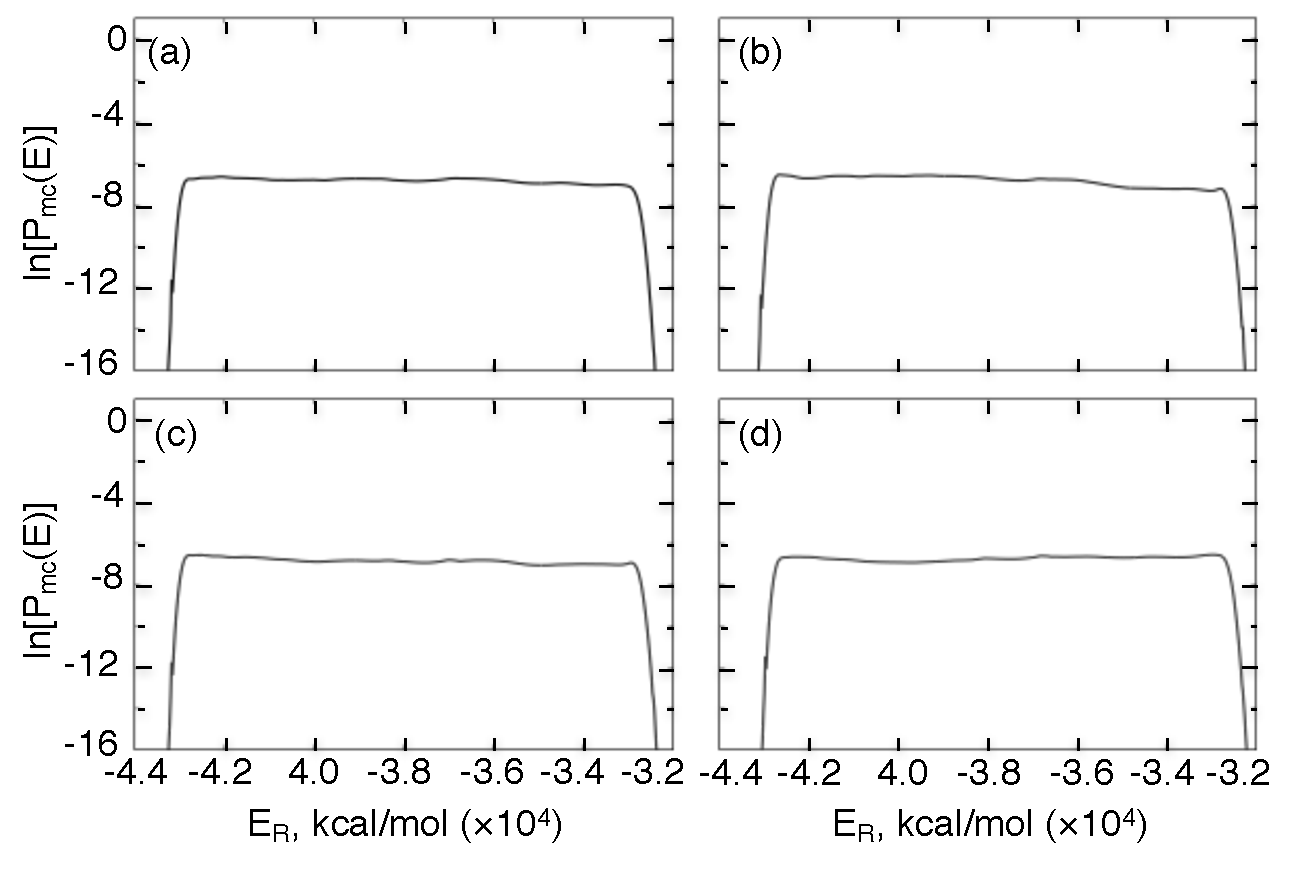
\includegraphics[width=10cm]{../single_CTD/figures_p53ctd/2.pdf}
  \caption{\label{fig:P_vmc_p53} Flat energy distribution for the a) NonAc(H+), b) Ac(H+), c) NonAc, and d) Ac systems. 
Individual distributions ($P_{\rm vmc}(E_{\rm R},v_i), i=1,..,n_{\rm vs}$) for the virtual states are integrated into the shown distribution $P_{\rm mc}(E_{\rm R})$ using the method presented in an earlier report.[3]}
\end{figure}

\subsection{Free energy landscape of the full-length fragments}
Figure \ref{fig:fel_whole} shows FELs at 300 K constructed in the 2D PCA space. The contribution ratios $rc_1$ and $rc_2$ from $Q_{\rm sum}$ were, respectively, 41.4\% and 18.8\%. Then the contributions from the PC 1 and 2 axes ($rc_1+rc_2$) were 60.2\%. In Figure \ref{fig:fel_whole}, we refer to the clusters as $G^{\rm SYS}_k$, where superscript SYS specifies the computed system and the subscript $k$ is a label assigned to the clusters. Figure \ref{fig:fel_whole_confs} demonstrates representative tertiary structures in each cluster. In all panels, $G^{\rm SYS}_1$ is assigned to the cluster of the global minimum PMF, which corresponds to a nearly complete helix (see structures in $G^{\rm SYS}_1$ in Figure 4) located at the same position in the 2D PCA space. Figure \ref{fig:fel_whole} manifests that the clusters can transition mutually at 300 K: the free-energy barriers among the clusters are surmountable at 300 K, except for the cluster $G^{\rm NonAc(H^+)}_4$. In other words, the CTD fragments are disordered.

\begin{figure}
  \centering
  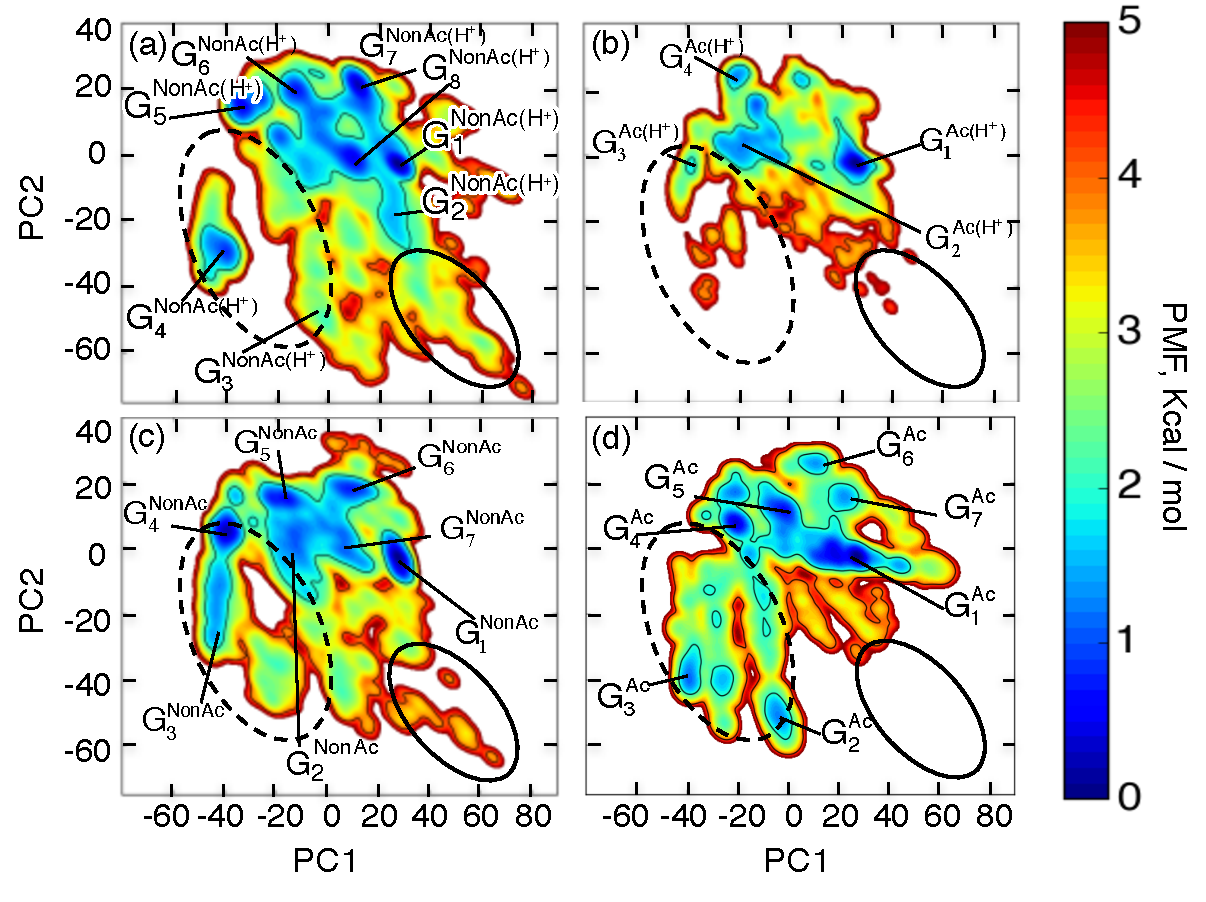
\includegraphics[width=10cm]{../single_CTD/figures_p53ctd/3.pdf}
  \caption{\label{fig:fel_whole}}
\end{figure}

\begin{figure}
  \centering
  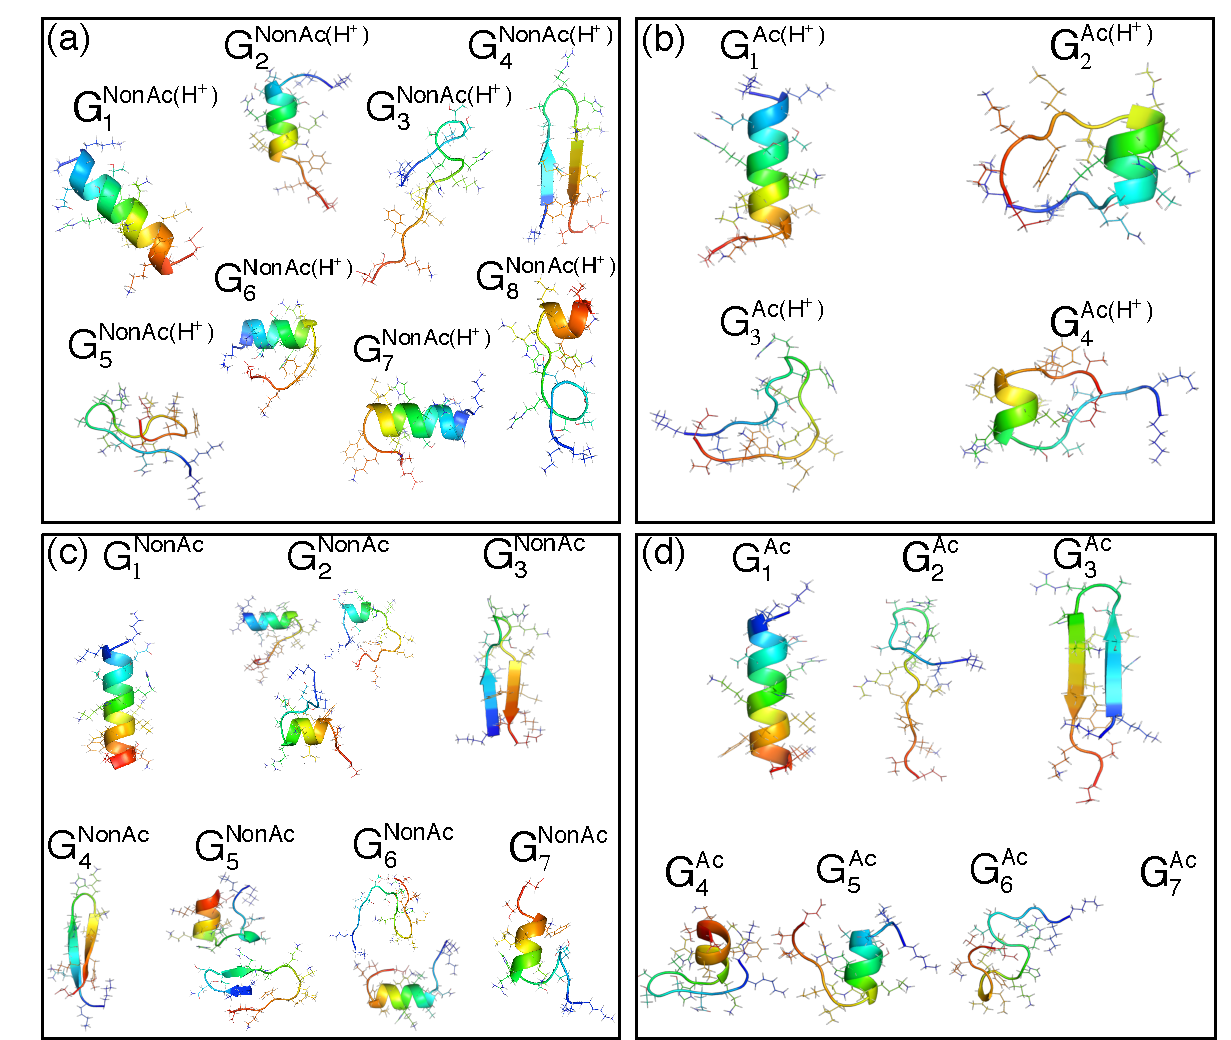
\includegraphics[width=10cm]{../single_CTD/figures_p53ctd/4.pdf}
  \caption{\label{fig:fel_whole_confs}}
\end{figure}

All FELs involved not only the complete-helix cluster ($G^{\rm SYS}_1$) but also partially helical ones. The tertiary structures are shown in $G^{\rm NonAc(H^+)}_2$, $G^{\rm NonAc(H^+)}_6$, $G^{\rm NonAc(H^+)}_7$, and $G^{\rm NonAc(H^+)}_8$ in Figure \ref{fig:fel_whole_confs}a, in $G^{\rm Ac(H^+)}_2$ and $G^{\rm Ac(H^+)}_4$ in Figure \ref{fig:fel_whole_confs}b, in $G^{\rm NonAc}_2$, $G^{\rm NonAc}_5$, $G^{\rm NonAc}_6$, and $G^{\rm NonAc}_7$ in Figure \ref{fig:fel_whole_confs}c, and in $G^{\rm Ac}_4$, $G^{\rm Ac}_5$, and $G^{\rm Ac}_7$ in Figure \ref{fig:fel_whole_confs}d. The $\beta$-hairpins are also found as $G^{\rm NonAc(H^+)}_4$ in Figure \ref{fig:fel_whole_confs}a, as $G^{\rm Ac(H^+)}_3$ in Figure \ref{fig:fel_whole_confs}b (this is a distorted hairpin-like structure), as  $G^{\rm NonAc}_3$, $G^{\rm NonAc}_4$, and $G^{\rm NonAc}_5$ in Figure \ref{fig:fel_whole_confs}c, and as $G^{\rm Ac}_3$ in Figure \ref{fig:fel_whole_confs}d.

Although all the CTD fragments exhibited conformational diversity, the FEL shape is considerably different as shown in Figure \ref{fig:fel_whole}. Remarkable differences are apparent for regions indicated by the solid-line and broken-line circles in the figure. Comparison of FELs between Figures \ref{fig:fel_whole}a and \ref{fig:fel_whole}b as well as between Figures \ref{fig:fel_whole}c and \ref{fig:fel_whole}d clarifies that the acetylation of K382 diminishes the probability in the region by a solid-line circle. We find that extended conformations are distributed in the solid-line circled region. It is likely that the acetylation facilitates hydrophobic-core formation by making the CTD fragment compact, which results in disappearance of the extended conformations. To verify this expectation, we calculated a radius of gyration of the fragments at 300 K only using hydrophobic atoms in the CTD fragment: C$\beta$, C$\gamma$, and C$\delta$ atoms of K372, K373, K381, K382, and K386; C$\beta$ atom of H380; C$\beta$ atom of L383; C$\beta$ atom of M384; and C$\beta$ atom of P385. The side-chain tip of the acetylated K382 in the Ac(H+) and Ac systems was excluded from the computation of radius of gyration for the strict comparison because the side-chain tip does not exist in NonAc(H+) and NonAc. Table 3 presents the radius of gyration values ($R_{\rm g}$), which demonstrates that the acetylation induces a compact hydrophobic core. We discuss this point further by viewing the tertiary structures of the CTD fragments below.

We computed the secondary-structure propensity of each residue in $Q_{\rm SYS}$ using the DSSP program.[47] Figure \ref{fig:ss_contents_p53} depicts the secondary-structure contents along the sequence at 300 K. Comparison of Figures \ref{fig:ss_contents_p53}a and \ref{fig:ss_contents_p53}b reveals that K382 acetylation induces the helix propensity of the CTD fragment. This tendency is also apparent from comparison of Figures \ref{fig:ss_contents_p53}c and \ref{fig:ss_contents_p53}d. Furthermore, Table 4 presents the helix increment by the acetylation quantitatively.

\begin{figure}
  \centering
  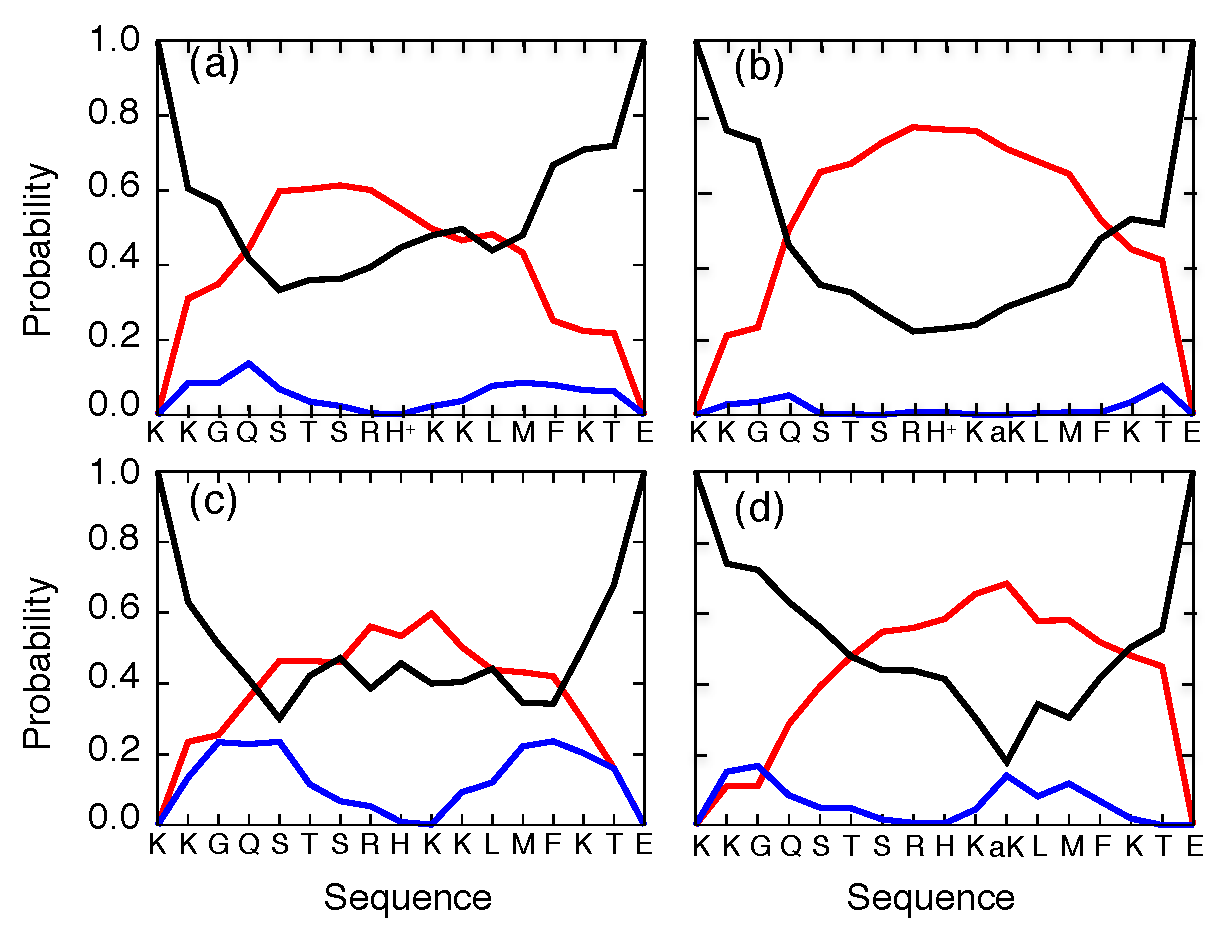
\includegraphics[width=10cm]{../single_CTD/figures_p53ctd/5.pdf}
  \caption{\label{fig:ss_contents_p53}}
\end{figure}

Figure \ref{fig:repres_struct_in_G}a presents a tertiary structure taken from the cluster $G^{\rm Ac(H^+)}_1$, where the aK382 and L383 side-chains form a hydrophobic contact in the helix. Similarly, a conformation taken from $G^{\rm Ac}_1$ shows that a hydrophobic contact is formed between aK382 and S378 (Figure 6b). Figure \ref{fig:repres_struct_in_G}c shows a hydrophobic contact between the side-chain stems of aK382 and K381 in the partially helical conformation taken from $G^{\rm Ac(H^+)}_2$. Unless K382 is acetylated, a repulsive force acts between these two lysine residues. Furthermore, in this conformation, the oxygen atom in the aK382 side-chain and the nitrogen atom in the K381 side-chain interact electro-statistically. Figure \ref{fig:repres_struct_in_G}d presents a conformation taken from $G^{\rm Ac}_5$, where a hydrophobic core is formed by side-chain tips of aK382 and M384 and side-chain stem of R379. Consequently, the acetylation induces the hydrophobic core formation in helices. Then the radius of gyration becomes small. If Lys382 is non-acetyl form, then repulsion interactions take place between Lys382 and the other positively charged residues in the helix because each sequence of the fragments includes six or seven positively charged residues. Consequently, acetyl-lysine stabilizes helical structures more than non-acetyl lysine does.

\begin{figure}
  \centering
  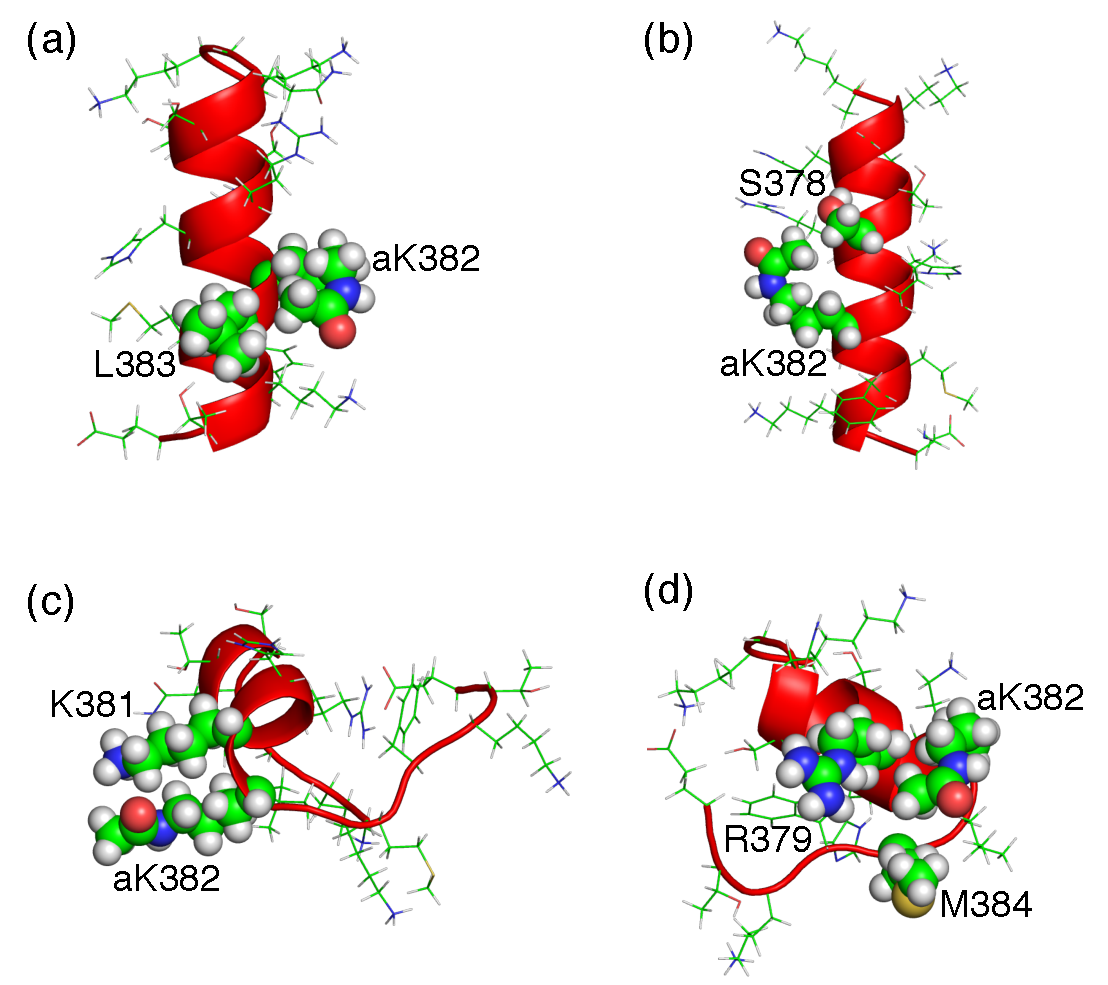
\includegraphics[width=10cm]{../single_CTD/figures_p53ctd/6.pdf}
  \caption{\label{fig:repres_struct_in_G}}
\end{figure}

As described above, comparison between Figures \ref{fig:fel_whole}a and \ref{fig:fel_whole}c as well as between Figures \ref{fig:fel_whole}b and \ref{fig:fel_whole}d clarified that the charge neutralization of H380 increases the probability in the broken-line circled region, where hairpin structures are distributed. Figure \ref{fig:ss_contents_p53} and Table 4 also show that the charge neutralization enhances the hairpin formation. Figure \ref{fig:haripin_confs_p53}a portrays a hairpin taken from cluster $G^{\rm NonAc}_4$, where H380 and K381 form a hydrogen bond. Repulsive interaction acts between H380 and K381 if H380 is positively charged. Similarly, Figure \ref{fig:haripin_confs_p53}b displays a distorted hairpin taken from $G^{\rm NonAc}_4$ @@WRONG?, where the side-chain of H380 and main-chain of K382 form a hydrogen bond. If H380 is positively charged, then this distorted hairpin becomes unstable because a repulsive interaction between the positively charged H380 and K382 might break the hydrogen bond. Furthermore, a repulsive interaction between the positively charged H380 and R379 might also destabilize the $\beta$-hairpin structure. Consequently, the charge neutralization of H380 is necessary for stabilizing the hairpins in Figures \ref{fig:haripin_confs_p53}a and \ref{fig:haripin_confs_p53}b. Figure \ref{fig:haripin_confs_p53}c displays a hairpin from $G^{\rm NonAc}_3$, where H380 and T377 form a hydrogen bond. These tertiary structures exemplify that the charge neutralized H380 serves the hydrogen bonds to stabilize turns in the hairpins.

\begin{figure}
  \centering
  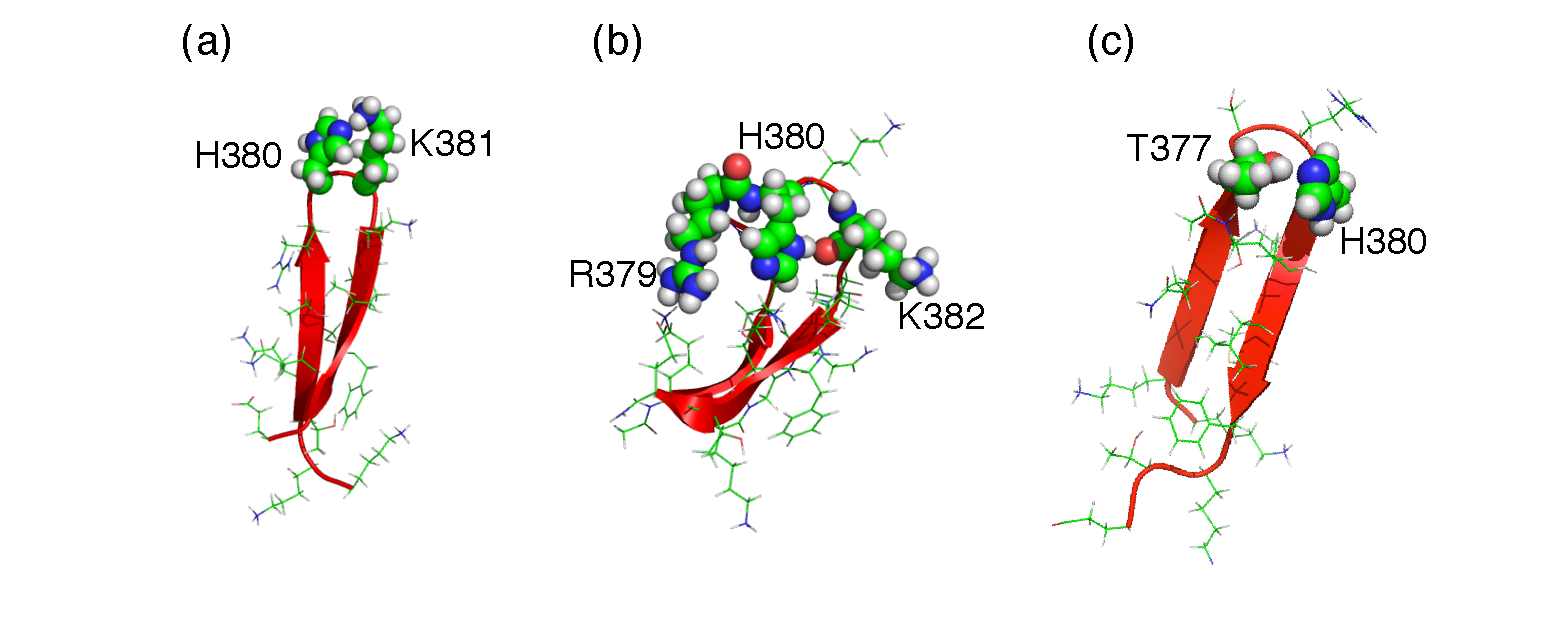
\includegraphics[width=10cm]{../single_CTD/figures_p53ctd/7.pdf}
  \caption{\label{fig:haripin_confs_p53}}
\end{figure}

Data shown in the figure \ref{fig:fel_whole} suggest visually that the Ac(H+) system might have the narrowest structural varieties among the four systems. To elucidate this feature quantitatively, we computed the standard deviation $\sigma_{\rm SYS}$ of the conformational distribution for C$\alpha$ atoms for each system as
\begin{equation}
\label{eq:sig_ca}
\sigma_{\rm SYS} = \sum_i [<q_i^2 > - <q_i>^2]^{1/2},
\end{equation}
where the brackets are the ensemble average over conformations in each ensemble $Q_{\rm SYS}$ weighted at 300 K. The resultant values are: $\sigma_{\rm NonAc(H^+)}= 37.6 \AA $,  $\sigma_{\rm Ac(H^+)}= 30.6 \AA $,  $\sigma_{\rm NonAc}= 36.5 \AA $, and  $\sigma_{\rm Ac}= 36.9 \AA $. These values of structural fluctuations are consistent with the radii of gyration in Table 3. Consequently, the Ac(H+) system has the smallest standard deviation. This reduction of the broadening results from the acetylation of K382. One might expect the Ac system to have a narrow distribution because K382 is also acetylated in this system. However, as shown above, the neutralization of H380 induces hairpins, which prevents reduction of the distribution.

A temperature replica exchange MD simulation[24, 26] of a 14-residue p53 CTD fragment and a conventional MD simulation[24, 26] of a 15-residue p53 CTD fragment were performed to obtain a conformational ensemble in the unbound state. These two fragments are fully included in our 17-residue fragment, and H380 and K382 were positively charged respectively and K382 was non-acetylated. Consequently, those fragments are parts of the NonAc(H+) fragment, and binds to the S100B molecule with adoption of a helical conformation. It is particularly interesting that, in these studies, the ensembles involved a helical fraction, which is consistent with our result for $Q_{\rm NonAc(H^+)}$. In contrast, recent CD measurement of two 32-residue p53 CTD fragments, which involve our NonAc and Ac segments, showed that the conformations of the CTD fragments are randomized.[48] Our computational results demonstrated that both $Q_{\rm NonAc}$ and $Q_{\rm Ac}$ contain a helical fraction and that the helical content of $Q_{\rm Ac}$ is larger than that of $Q_{\rm NonAc}$. This apparent inconsistency between the computational results and the CD-experimental observation should be analyzed. We note, however, that the fragment length for the CD experiment is considerably longer than ours.

To link the computation and experiment, we conducted CD experiments of the NonAc and Ac fragments of 17 residues long. TFE enhances formation of secondary structures, especially of helix.[49, 50] To clarify the inherent helix propensity of the two fragments, the measurement was done at various TFE concentrations. CD spectra at zero TFE concentration have suggested that the overall structural feature of both fragments is characterized by a disorder state (data not shown), which is consistent to the preceding CD measurement.[48] Therefore, the helical contents obtained from the simulations were larger than those from the CD experiments. In fact, although CD experiments are useful to discuss the secondary-structure properties of polypeptide qualitatively, the CD data might involve quantitative ambiguity in assessing the secondary-structure contents. On the other hand, the simulation data might involve some errors. Therefore, we compare the simulation data with the CD data qualitatively. Figure \ref{fig:TFE_mesure} shows that the Ac fragment has a higher helix contents than the NonAc fragment at all examined TFE concentrations including the zero TFE concentration. This result was also supported by analysis of the CD spectra using “Bestsel” software [51] (data not shown), which estimates the secondary-structure contents from CD spectra. Therefore, we conclude from both computation and experimentation that the acetylation of K382 enhances the helix formation slightly.

\begin{figure}
  \centering
  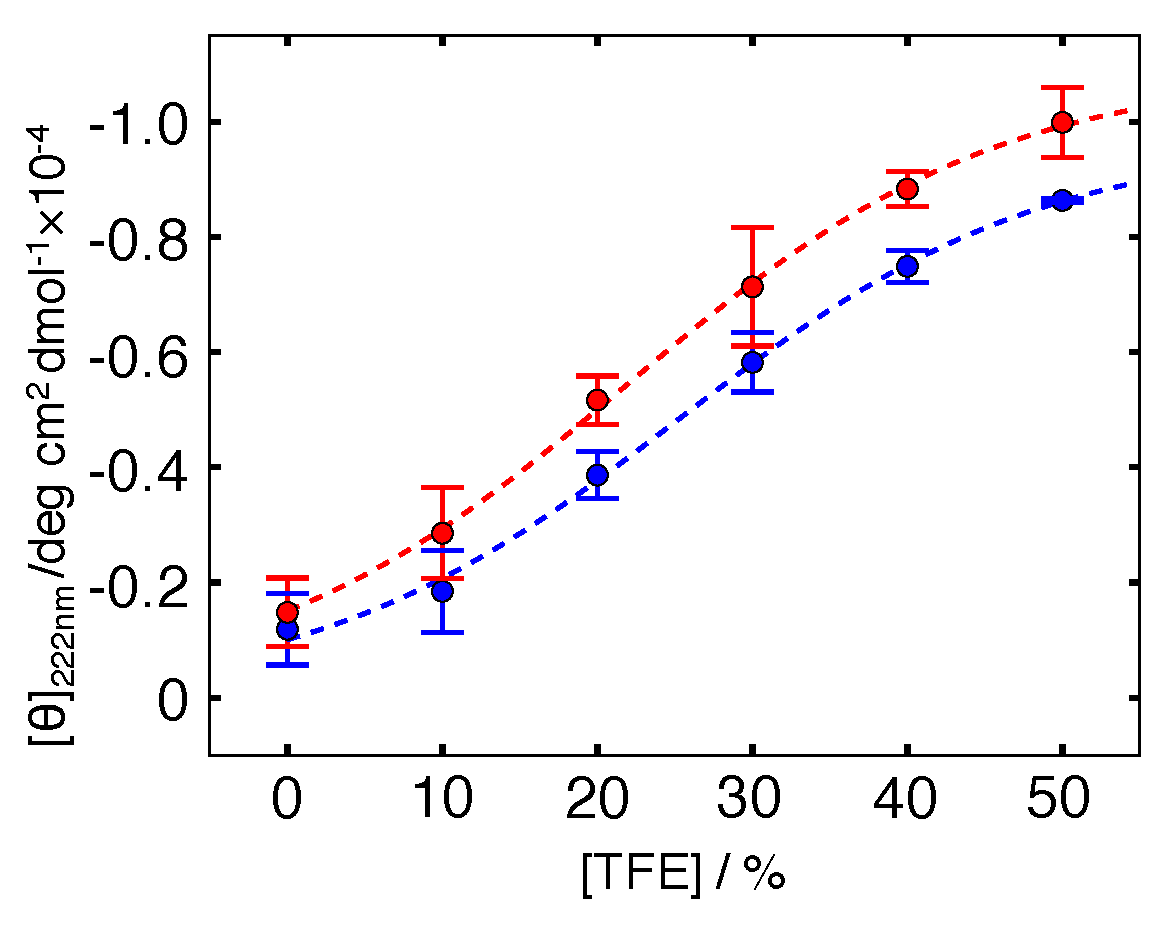
\includegraphics[width=10cm]{../single_CTD/figures_p53ctd/8.pdf}
  \caption{\label{fig:TFE_mesure}}
\end{figure}

As described earlier, NonAc(H+) binds to S100B with adopting helical conformation and Ac(H+) does not adopt a helical conformation to bind to a partner (Table 1). This experimentally obtained result might be inconsistent to the computational result that $Q_{\rm NonAc(H^+)}$ contains a smaller helix content than $Q_{\rm NonAc(H^+)}$. We discuss possible binding mechanisms of the CTD fragments to their partner molecules in the next section.

\subsection{Free energy landscape of the common binding region}
As described in the Introduction section, the p53 CTD has a hub property. Four CTD-partner complex structures were determined. As described in the Materials and methods section, the residues 380–386 of CTD are the common binding region to all the four partners S100B, Sir2, CBP, and Cyclin A. We computed the 2D FEL for this common binding region (Figure \ref{fig:fel_common}), where the variance-covariance matrix was computed only for the common binding region. This figure shows that various clusters are distributed in the 2D PCA space for all the ensembles. The contribution ratios are  $rc_1$=73.5 \% and $rc_2$= 14.4 \%; then $rc_1+rc_2$=87.9 \%.

\begin{figure}
  \centering
  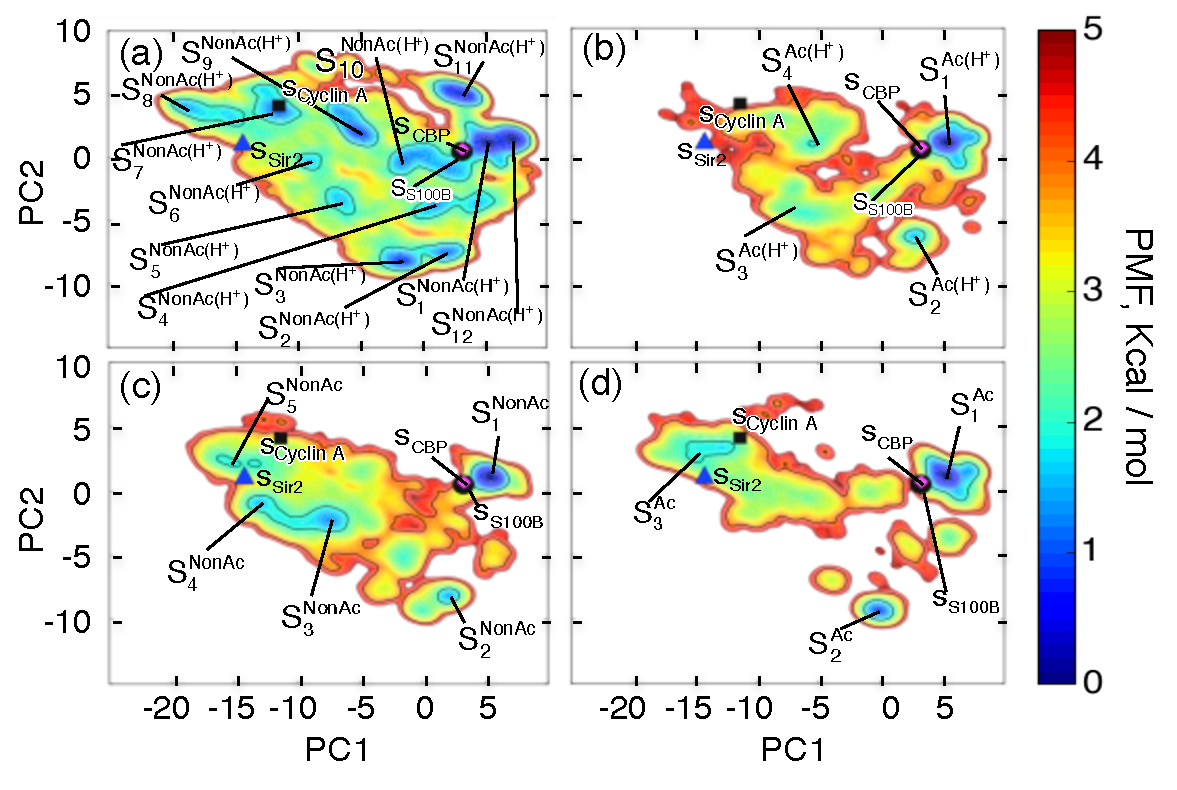
\includegraphics[width=10cm]{../single_CTD/figures_p53ctd/9.pdf}
  \caption{\label{fig:fel_common}}
\end{figure}

We refer to the clusters as $S_k^{\rm SYS}$, where superscript SYS specifies the computed system and subscript  is a label assigned to clusters in Figure \ref{fig:fel_common}. Cluster $S_1^{\rm SYS}$ is assigned to the global minimum of PMF in all panels along with FEL for the full-length fragments. Figure \ref{fig:repre_confs_comm_fel} presents representative tertiary structures in each cluster. Again, this cluster corresponds to a helical cluster (see structures in $S_1^{\rm SYS}$ in the figure \ref{fig:repre_confs_comm_fel}) located at the same position in all panels.

\begin{figure}
  \centering
  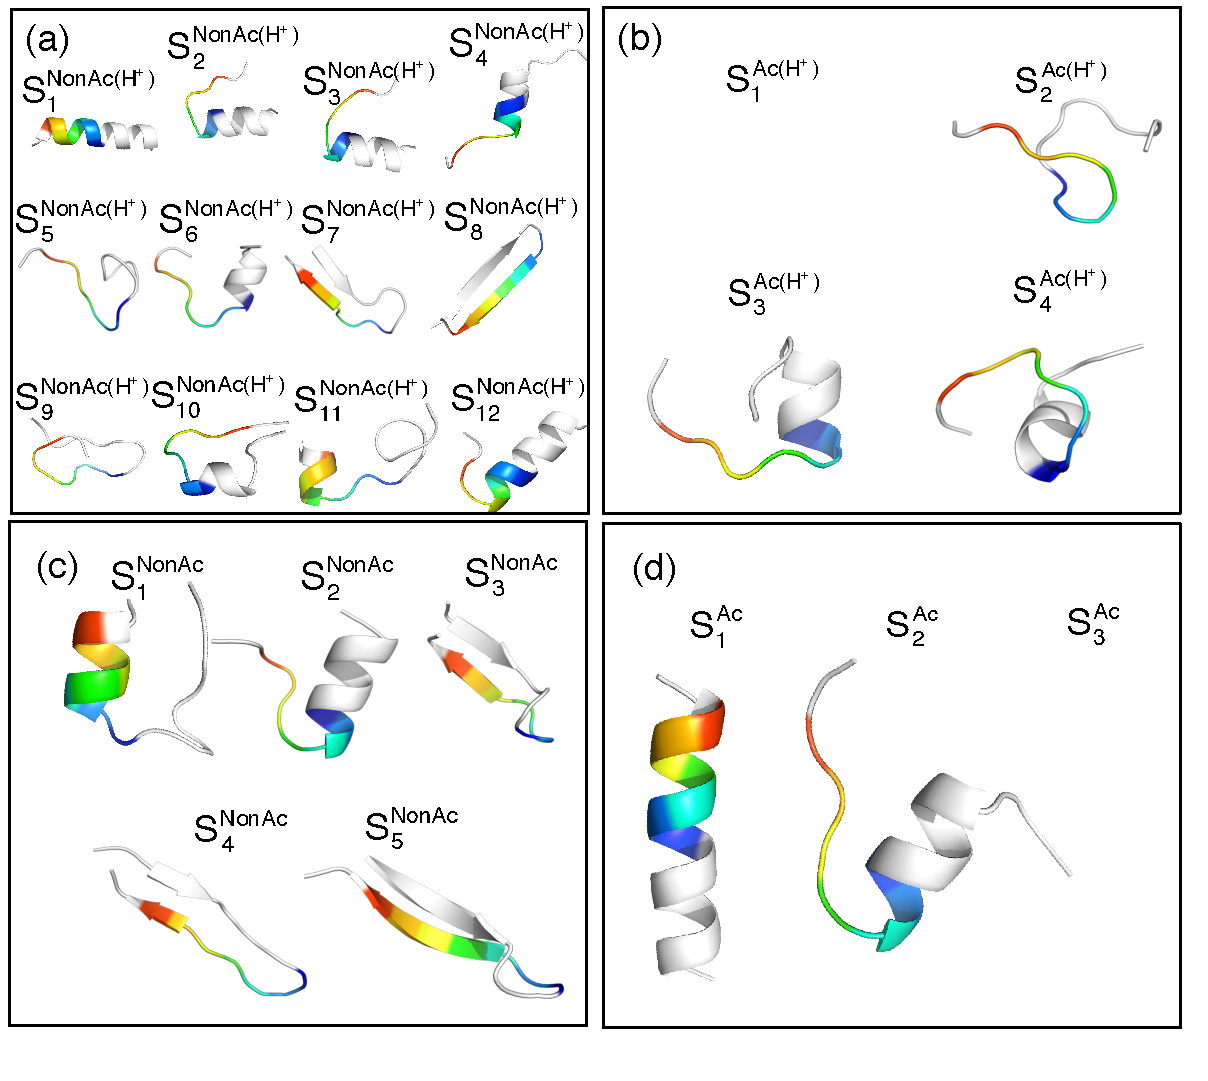
\includegraphics[width=10cm]{../single_CTD/figures_p53ctd/10.pdf}
  \caption{\label{fig:repre_confs_comm_fel}}
\end{figure}

Apparently, the ensemble $Q_{\rm NonAc(H^+)}$ has the broadest distribution of the four ensembles. 
Many clusters are found in FEL (Figure \ref{fig:fel_common}a). 
The tertiary structures taken from the clusters are diverse (Figure \ref{fig:repre_confs_comm_fel}a): 
The complete helix is $S_1^{\rm NonAc(H^+)}$; 
partial helices are $S_2^{\rm NonAc(H^+)}$, $S_3^{\rm NonAc(H^+)}$, $S_4^{\rm NonAc(H^+)}$, $S_6^{\rm NonAc(H^+)}$, $S_{10}^{\rm NonAc(H^+)}$, $S_{11}^{\rm NonAc(H^+)}$, and $S_{12}^{\rm NonAc(H^+)}$; 
$\beta$ hairpins are $S_7^{\rm NonAc(H^+)}$ and $S_8^{\rm NonAc(H^+)}$; and random-coiled structures are $S_5^{\rm NonAc(H^+)}$ and $S_9^{\rm NonAc(H^+)}$. 
Inter-cluster transitions can take place readily because free-energy barriers among the clusters are low.

Structural diversity decreases when K382 is acetylated and/or H380 is neutralised. 
In $Q_{\rm Ac(H^+)}$, no $\beta$ hairpin cluster exists, although three partial helix clusters ($S_1^{\rm NonAc(H^+)}$, $S_3^{\rm Ac(H^+)}$ and $S_4^{\rm Ac(H^+)}$) do (Figure \ref{fig:fel_common}b).
In $Q_{\rm NonAc}$, only two helix clusters ($S_1^{\rm NonAc}$ and $S_2^{\rm NonAc}$) and three $\beta$ hairpin clusters ( $S_3^{\rm NonAc}$,  $S_4^{\rm NonAc}$ and  $S_5^{\rm NonAc}$) exist (Figure \ref{fig:fel_common}c).
In $Q_{\rm Ac}$, two helix clusters ($S_1^{\rm Ac}$ and $S_2^{\rm Ac}$) exist, but no hairpin cluster exists (Figure \ref{fig:fel_common}d).
In fact, the free-energy barriers among clusters in Figures \ref{fig:fel_common}b, \ref{fig:fel_common}c, and \ref{fig:fel_common}d are higher than those in Figure \ref{fig:fel_common}a. 
Therefore, inter-cluster transitions in Figures \ref{fig:fel_common}b, \ref{fig:fel_common}c, and \ref{fig:fel_common}d occur by passing narrower regions than those in Figure \ref{fig:fel_common}a. 
Figure \ref{fig:comp_structs} displays the experimentally determined complex structures and sampled conformations that are located near the bound form in the free-energy landscape (Figure \ref{fig:fel_common}). 
Apparently, the sampled conformations closely resemble the experimental bound form.
\begin{figure}
  \centering
  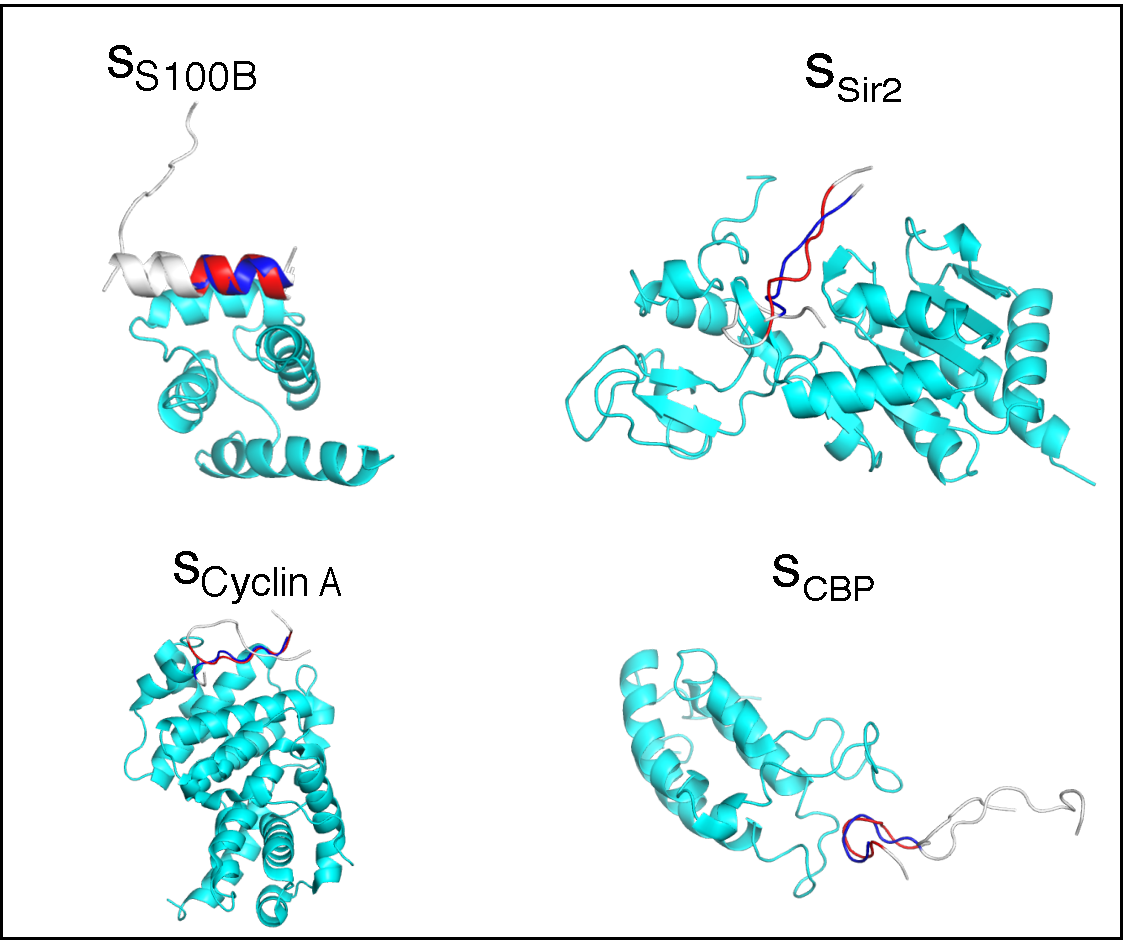
\includegraphics[width=10cm]{../single_CTD/figures_p53ctd/11.pdf}
  \caption{\label{fig:comp_structs}}
\end{figure}

The bound forms of the common binding region in the experimentally determined complex structures are also assigned to Figure \ref{fig:fel_common}. 
The bound forms $\rm s_{S100B}$ and $\rm s_{CBP}$ are mutually close depicted in Figure \ref{fig:fel_common} although $\rm s_{S100B}$ and $\rm s_{CBP}$ respectively denote a helix and a twisted conformation (See Fig. S1 of Supplementary Materials). 
The closeness of the two conformations results from the similarity of the C$\alpha$ atomic pair distances. 
Remember that the PCA space is generated based on the inter-C$\alpha$ atomic distances. 
Therefore, $\rm s_{CBP}$ can convert to $\rm s_{S100B}$ by minor rearrangements of the C$\alpha$ atomic pair distances.
Figure \ref{fig:fel_common} proposes possible mechanisms of CTD binding to their partner molecules. 
We infer that the main binding mechanism of NonAc(H+) to S100B is the population selection because $\rm s_{S100B}$ is located at a fringe of the most stable cluster $S_1^{\rm NonAc(H^+)}$ (Figure \ref{fig:fel_common}a). 
In other words, $\rm Q_{NonAc(H^+)}$ prepares the bound form in advance. 
Furthermore, because the free-energy barriers from the other clusters to $S_1^{\rm NonAc(H^+)}$ are low as described above, the bound form is recruited quickly when the bound form is exhausted to bind to S100B. 
The helical content of $\rm Q_{NonAc(H^+)}$ is smaller than that of $\rm Q_{Ac(H^+)}$. 

Figure \ref{fig:fel_common}a suggests that $\rm Q_{NonAc(H^+)}$ contains helical conformations sufficient for use for binding to S100B even if the helical content of $\rm Q_{NonAc(H^+)}$ is less than that of $\rm Q_{Ac(H^+)}$.

The population-selection mechanism might take place when the Ac fragment binds to CBP, where the conformations in the most stable cluster $S_1^{\rm Ac}$ can transition readily to the conformation $\rm s_{CBP}$ (Figure \ref{fig:fel_common}d). 
However, the cluster $S_1^{\rm Ac}$ is not connected to the other clusters by low free-energy pathways. 
Consequently, the recruitment of conformations to  from the other clusters might be slow. 
In other words, the rate constant for the Ac fragment binding to CBP might be smaller than that for the NonAc(H+) binding to S100B if the population-selection mechanism occurs.

For binding of the Ac(H+) fragment to Sir2, the conformation $\rm s_{Sir2}$ is located at a high free-energy site in Figure \ref{fig:fel_common}b. 
Therefore, we presume that the fragment binds to Sir2 with a different conformation than $\rm s_{Sir2}$, by which an encounter complex is formed. 
Then, the intermolecular interactions bring the fragment to the genuine complex structure. 
Therefore, we presume that the binding mechanism of this fragment belongs to the induced folding mechanism.

The NonAc fragment can bind to either S100B or Cyclin A (Table 1). The binding mechanism to S100B might be the population selection for the same reason for the NonAc(H+) fragment binding to S100B. 
The structure $\rm s_{Cyclin}$ is located at a site with free energy of about 3 kcal / mol in Figure \ref{fig:fel_common}c. 
Therefore, a small fraction of the ensemble $\rm Q_{NonAc}$ is a conformation close to $\rm s_{Sir2}$. Consequently, the binding mechanism of this fragment to Cyclin A might belong to the population selection. However, the main fraction of $\rm Q_{NonAc}$ is far from $\rm s_{Cyclin}$. Therefore, different conformations might be used to bind to Cyclin A. Consequently, the induced folding mechanism is also possible.

It is likely that the diversity of FEL modulated by the state variation of lysine and/or histidine induces the hub property of CTD. One can reasonably infer that different FELs have different interaction mechanisms to other molecules. A single protein segment can have multiple binding partners. This property is called a hub. It is noteworthy that the flexibility of the CTD segment is fundamentally important for the diversity of FEL. If CTD is a structurally well-defined portion of the protein, then FEL has no great diversity. Therefore, CTD might bind only to a single partner.

The binding mechanism proposed here is based only on the FEL of the unbound state, which means that no IDR-partner interactions are considered. 
To ascertain whether the proposed mechanism is correct or not, we should perform simulations of systems where CTDs and their partner molecules coexist, as in earlier studies.[11,32] 
However, the current study is useful to investigate the variation of FEL in the presence or absence of the partner.

Finally, we confirmed the convergence of the sampled data. As reported in the convergence of sampling–section in Supplementary Materials, the convergence is good for all the systems.

\subsection{Conclusions}
To investigate a highly flexible biomolecular system, computational approaches are fundamentally important because experimental detection of large fluctuations at an atomistic resolution is still difficult. 
Because the high flexibility is an inherent property of IDR, investigation of the conformational ensemble is necessary to elucidate the nature of IDR. 
Therefore, a powerful conformational sampling method is required. 
We performed the enhanced conformational sampling method, V-McMD, to obtain the conformational ensembles of four p53 CTD fragments in the unbound state at the atomic resolution in an explicit solvent. 
@@@Then we constructed free-energy landscapes from the obtained conformational ensembles.

The shape of the free-energy landscape varied depending on the K382 acetylation and/or the H380 neutralization in CTD. 
It is particularly interesting that acetylation enhanced the helix propensity. This computational result was confirmed using CD experiments. 
We also demonstrated that acetylation induces the hydrophobic-core formation. The H380 neutralization has enhanced the hairpin formation of CTD. 
The helix content obtained from V-McMD tends to be larger than that from the CD experiment. 
This fact suggests that the force field is imperfect and that there have not been accurate force fields yet.[52] Results from the CD experiment were explained by the McMD simulation with atomistic details. 
Therefore, we believe that our results are useful to discuss the variation of CTD’s conformational ensemble. 
Furthermore, the current results might assist in the generation of a general model for understanding the switching mechanism conducted by PTMs.

Each of the four CTD fragments has particular binding partner(s). 
We proposed possible binding mechanisms from the free-energy landscape of the unbound state. 
To judge whether the proposed mechanisms are correct or not, sampling of systems consisting of CTD and their partners is necessary for the next stage of research. 
However, as discussed in the Introduction, the binding mechanism of IDR is determined not only by the finally formed complex structure but also by the conformational distribution in the single-chain state. 
As discussed in Results, the spreading of the free-energy landscape and the free-energy barriers might affect the IDR-partner binding mechanism. 
Therefore, results of the current study of the unbound state are expected to be useful to investigate the variation of the free-energy landscape in the presence of the partner molecules. 
The results will provide useful knowledge to ascertain the hub property and coupled folding and binding of CTD.

\bibliography{/Users/siida/Dropbox/Bibliography/library}

\begin{appendices}
	\chapter{test}
\end{appendices}

\end{document}
